
\PassOptionsToPackage{table}{xcolor}
\documentclass{article}

\usepackage[francais]{babel}
\usepackage[T1]{fontenc}
\usepackage[utf8]{inputenc}
\usepackage{xcolor}
\usepackage{graphicx}
\usepackage[colorlinks=true]{hyperref}
\hypersetup{urlcolor=blue,linkcolor=red,colorlinks=false} 
\usepackage{algorithm,algorithmic}
\usepackage{listings}
\usepackage{amssymb}
\usepackage{setspace}
\usepackage{listings}
\usepackage{lscape}
\usepackage{amsmath}
\usepackage[margin=2.5cm]{geometry}


% Romain
\newcommand{\cRM}[1]{\MakeUppercase{\romannumeral #1}}  % Capital
\newcommand{\cRm}[1]{\textsc{\romannumeral #1}} % Petit majuscule
\newcommand{\crm}[1]{\romannumeral #1}
% Siècle %
\newcommand{\siecle}[1]{\cRM{#1}\textsuperscript{e}~siècle}


\definecolor{keywords}{RGB}{255,0,0}
\lstset{language=[LaTeX]TeX,
texcsstyle=*\color{keywords},
breaklines=true,
keywordstyle=\color{keywords},
commentstyle=\color{darkgreen},
tabsize=2,
backgroundcolor=\color{lightgrey},
escapeinside=||,
morekeywords={*,subsection,make title,tableofcontents,include graphics}
}


\rowcolors{1}{gray!25}{white}

\title{Les stratégies militaires dans les Systèmes Multi-Agents}
\author{Chloé Desdouits, William Dyce}
\date{\today}


\begin{document}

\maketitle

\tableofcontents
\newpage


\section{Organisations guerrières}
Il y a deux types d'organisations militaires bien différents : les armées et les guérillas. Nous allons présenter pour chaque type sa structure et le contexte dans lequel il existe.

\subsection{Armées}
Les armées sont des entités qui tirent leur légitimité de leur appartenance aux états ou jadis aux institutions religieuses.

\subsubsection{Structure}
La structure des armées est homogène : en effet, la hiérarchie est sous forme d'arbre dont les nœuds du même niveau ont le même nombre de fils.
\begin{figure}[H]
	\begin{centering}
	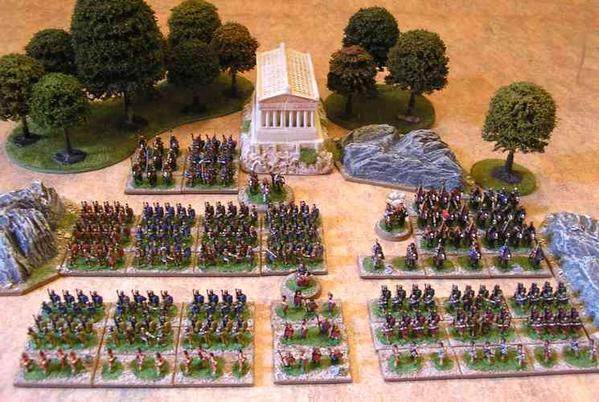
\includegraphics[width=0.8\linewidth]{../ressources/armee_cesar}
	\caption{Exemple d'organisation homogène de l'armée (armée de César - Warmaster ancients \cite{armee_de_cesar})}
	\end{centering}
\end{figure}

Cela permet de construire des formations à grande échelle qui aient une structure prédéfinie.
\begin{figure}[H]
\begin{centering}
\begin{tabular}{| c l | c l | c l | c l |}
	\hline
	\multicolumn{8}{| c |}{\textbf{Armée}}
	\\
	\multicolumn{2}{| c |}{\textbf{Spartiate}} 	& \multicolumn{2}{ c |}{\textbf{Romaine}} & \multicolumn{2}{ c |}{\textbf{Perse}}	& \multicolumn{2}{ c |}{\textbf{Mongole}} 	\\
	\hline
	 					&			& 					&			& 				&			& \textit{Ordu}		& > 10000			\\
	 \itshape Mora 			& 576		& \itshape Légion		& 6000		& \textit{Baivarabam}& 10000		& \textit{Tumen} 	& 10000			\\
	 \itshape Loche			& 144		& \itshape Cohorte		& 600		& \textit{Hazarabam}	& 1000		& \textit{Minghan}  	& 1000			\\
	 \itshape Pentécostye	& 72			& \itshape Manipule		& 200		& \textit{satabam}	& 100		& \textit{Zuut} 		& 100			\\
	 \itshape Énomotie		& 36			& \itshape Centurie		& 100		& \textit{Dathabam} 	& 10			& \textit{Arav} 		& 10				\\
	\hline
\end{tabular}
\caption{Effectif des unités dans différentes armées antiques \cite{mongol_army, spart_army, roman_legion,persian_army}}
\end{centering}
\end{figure}


\subsubsection{Contexte}
Les armées interviennent dans deux contextes principaux : la défense de la patrie et la conquête de nouveaux territoires.
\begin{figure}[H]
	\begin{centering}
	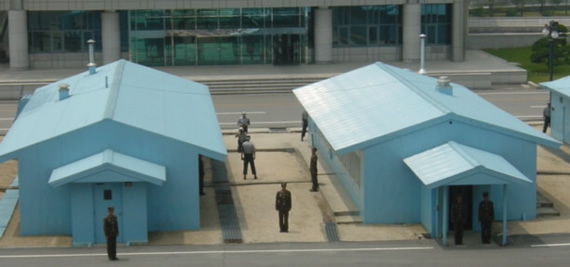
\includegraphics[width=\linewidth]{../ressources/dmz-corea}
	\caption{Zone démilitarisée entre la Corée du Sud et la Corée du Nord \cite{dmz_corea}}
	\end{centering}
\end{figure}
\begin{figure}[H]
	\begin{centering}
	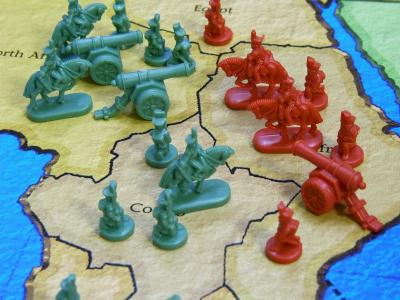
\includegraphics[]{../ressources/risk-board-game}
	\caption{Tentative de conquête dans le jeu Risk \cite{risk_picture}}
	\end{centering}
\end{figure}




\subsection{Guérillas}
Les guérillas se forment à la suite d'une scission idéologique entre le pouvoir en place et une partie de la population. Elles ont souvent à leur tête un leader charismatique.

\subsubsection{Structure}
Ces organisation sont souvent structurées de façon très hétérogène : peu de responsables et des formations à petite échelle.
\begin{figure}[H]
	\begin{centering}
	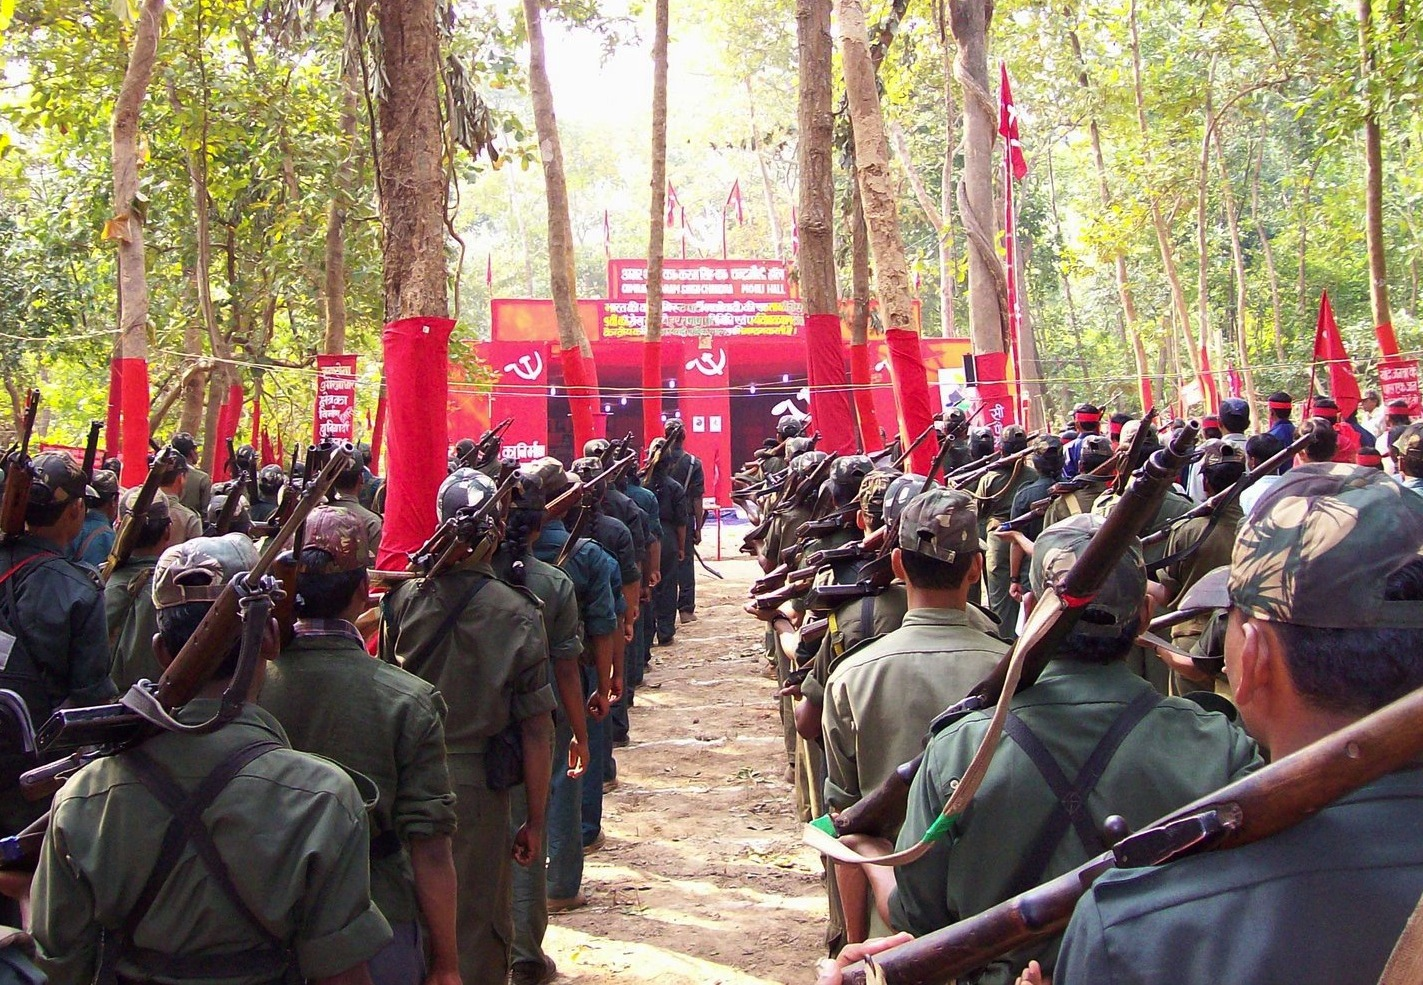
\includegraphics[width=\linewidth]{../ressources/guerrilla_naxalite}
	\caption{Guérilla Naxalite (Inde) \cite{guerrilla_naxalite}}
	\end{centering}
\end{figure}

Les guérillas, comme le montre la figure suivante, ont une échelle réduite par rapport aux forces contre lesquelles elles luttent.
\begin{figure}[H]
	\begin{centering}
	\begin{tabular}{| l | c | c | c | c |}
	\hline
	\textbf{Localisation}		& \textbf{Irlande} 	& \textbf{Inde} 	& \textbf{Cuba}	& \textbf{Colombie}	\\
	\hline
	\textbf{Régime}			& 55.000			& 1.414.000	& 35.000		& 300.000			\\
	\textbf{Insurgés}		& 15.000			& 15.000		& 200		& 20.000			\\
	\hline
	\end{tabular}
	\caption{Effectifs des forces du régime par rapport aux forces des guérillas \cite{naxalite_guerrilla_wiki, irish_civil_war_wiki}}
	\end{centering}
\end{figure}


\subsubsection{Contexte}
Les forces de guérilla sont adaptées au terrain : montagnes, maquis, villes \ldots
\begin{figure}[H]
	\begin{centering}
	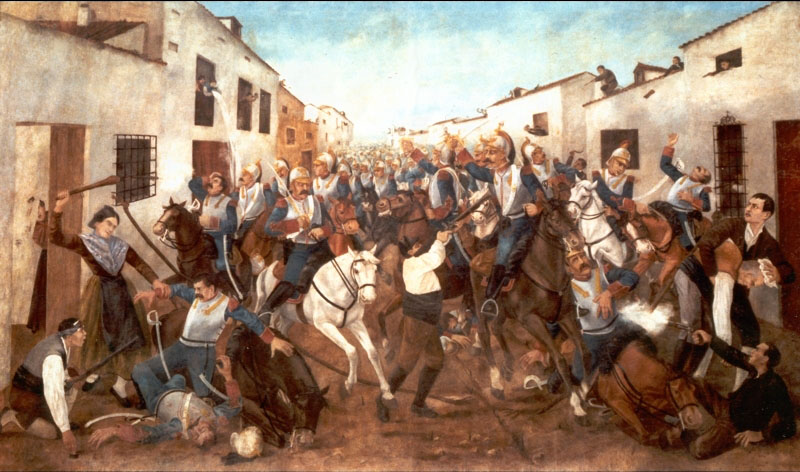
\includegraphics[width=\linewidth]{../ressources/valdepenas}
	\caption{Soulèvement de Valdepeñas ; guérilla urbaine \cite{valdepenas}}
	\end{centering}
\end{figure}
Elles sont mobiles.
\begin{figure}[H]
	\begin{centering}
	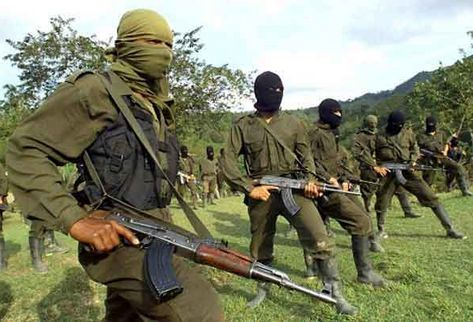
\includegraphics[]{../ressources/guerrilla_colombia}
	\caption{Guérilla colombienne \cite{guerrilla_colombia}}
	\end{centering}
\end{figure}
La plupart des recrues sont des civils.
\begin{figure}[H]
	\begin{centering}
	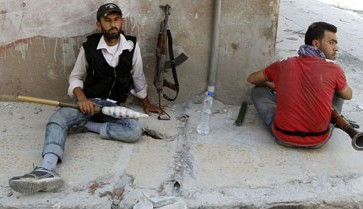
\includegraphics[]{../ressources/rebel_syrie}
	\caption{Des rebelles en Syrie \cite{rebel_syrie}}
	\end{centering}
\end{figure}


\section{Stratégies militaires}

\subsection{Définitions}
Politique \cite{politique_jomini}
\begin{quote}“La politique de la guerre c’est tout simplement décider où, quand, comment, avec quels alliés et pourquoi entrer en guerre.”\end{quote}
\begin{figure}[H]
	\begin{centering}
	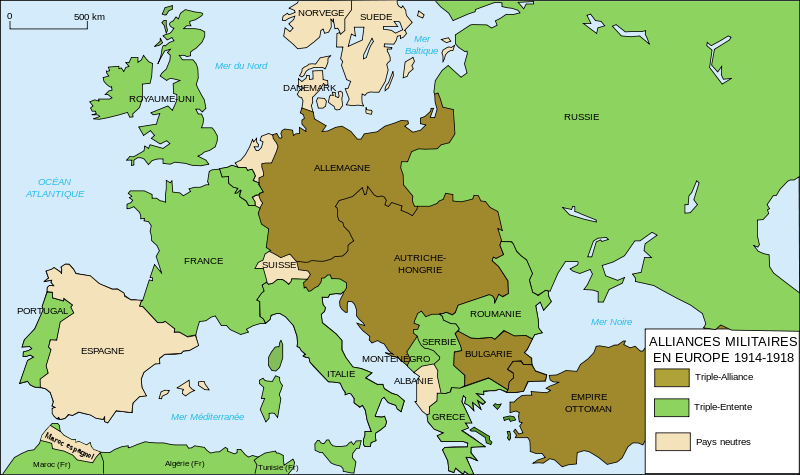
\includegraphics[width=\linewidth]{../ressources/alliances_ww1}
	\caption{Alliances militaires en Europe 1914-1918 \cite{ww1}}
	\end{centering}
\end{figure}

Stratégie \cite{military_strategy}
\begin{quote}“La stratégie militaire est l'art de coordonner -au plus haut niveau de décision- l'action de l'ensemble des forces militaires de la Nation pour conduire une guerre, gérer une crise ou préserver la paix.”\end{quote}
\begin{figure}[H]
	\begin{centering}
	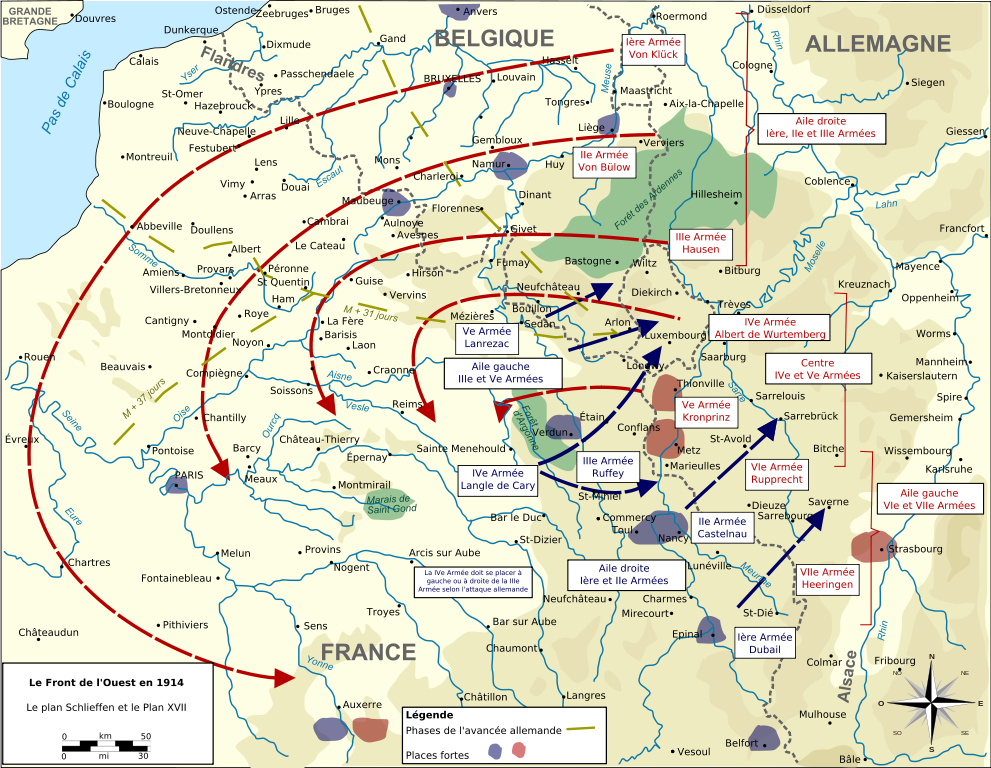
\includegraphics[width=\linewidth]{../ressources/strategy_ww1}
	\caption{Plans de bataille des états-majors allemand et français pendant la WW1 \cite{ww1}}
	\end{centering}
\end{figure}

Tactique \cite{tactic}
\begin{quote}“La tactique est l'art de diriger une bataille, en combinant, par la manœuvre, l'action des différents moyens de combat en vue d'obtenir le maximum d'efficacité.”\end{quote}
\begin{figure}[H]
	\begin{centering}
	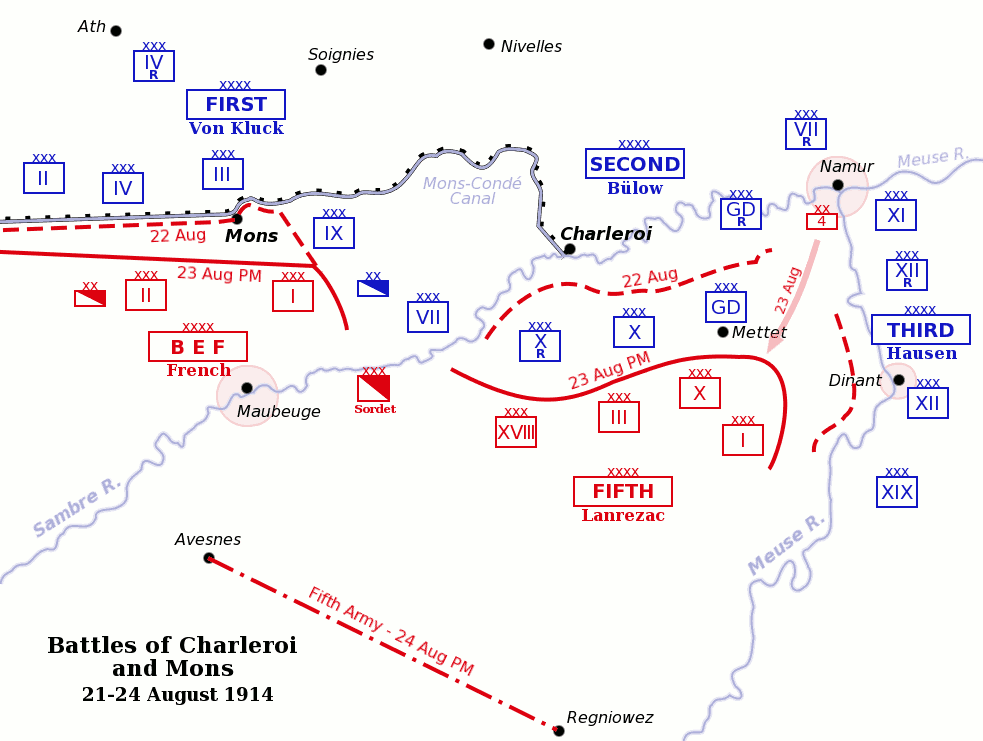
\includegraphics[width=\linewidth]{../ressources/Battles_of_Charleroi_ww1}
	\caption{Mouvement de troupes pendant la bataille de Charleroi (WW1) \cite{charleroi_battle}}
	\end{centering}
\end{figure}



\subsection{Stratégies}

\subsubsection{Sun Tzu}
Chine (\siecle{6} BC) \hfill \begin{minipage}{5cm}
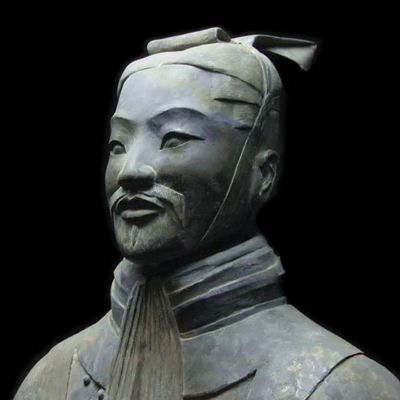
\includegraphics[width=\linewidth]{../ressources/sun_tzu_general}
\end{minipage}
\begin{quote}“L'art de la guerre, c'est de soumettre l'ennemi sans combat.”\end{quote}

Préceptes
\begin{itemize}
\item prendre toutes les possessions de l'adversaire et les conserver intactes
\item adaptabilité, préparation, connaissance du terrain et des forces en présence (espionnage)
\end{itemize}
Axes stratégiques
\begin{enumerate}
\item cause morale
\item conditions climatiques
\item conditions géographiques
\item qualités du dirigeant
\item organisation et discipline
\end{enumerate}

\cite{tzu1997art, sun_tzu_fighting, sun_tzu_wiki}

\subsubsection{Alexandre le grand}
Grèce (\siecle{4} BC)
\hfill \begin{minipage}{5cm}
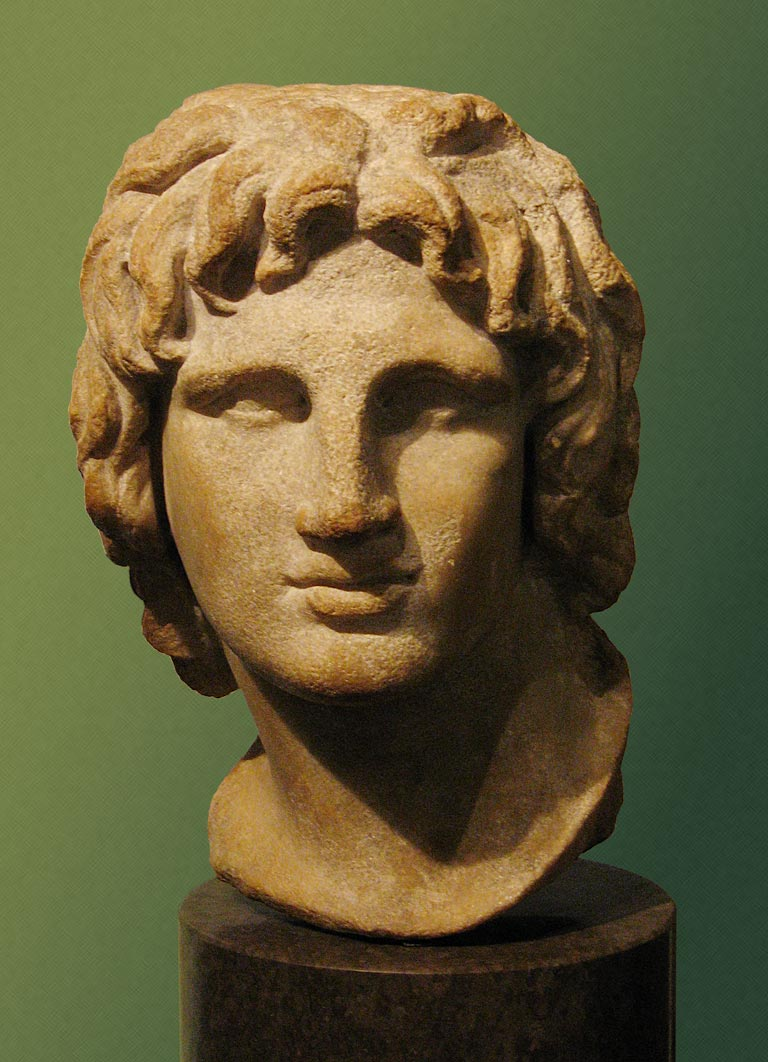
\includegraphics[width=\linewidth]{../ressources/AlexanderTheGreat_Bust}
\end{minipage}
\begin{quote}“Ce qui ne me tue pas me rend plus fort.”\end{quote}

Préceptes
\begin{itemize}
\item conscription et intégration des peuples vaincus
\item allègement de l'équipement des troupes
\end{itemize}
Axes stratégiques
\begin{enumerate}
\item assurer ses arrières
\item choisir judicieusement la voie d'accès pour chaque conquête
\end{enumerate}
\cite{alexander_the_great, alexandre_balkans}

\subsubsection{Julius Caesar}
Italie (\siecle{1} BC)
\hfill \begin{minipage}{5cm}
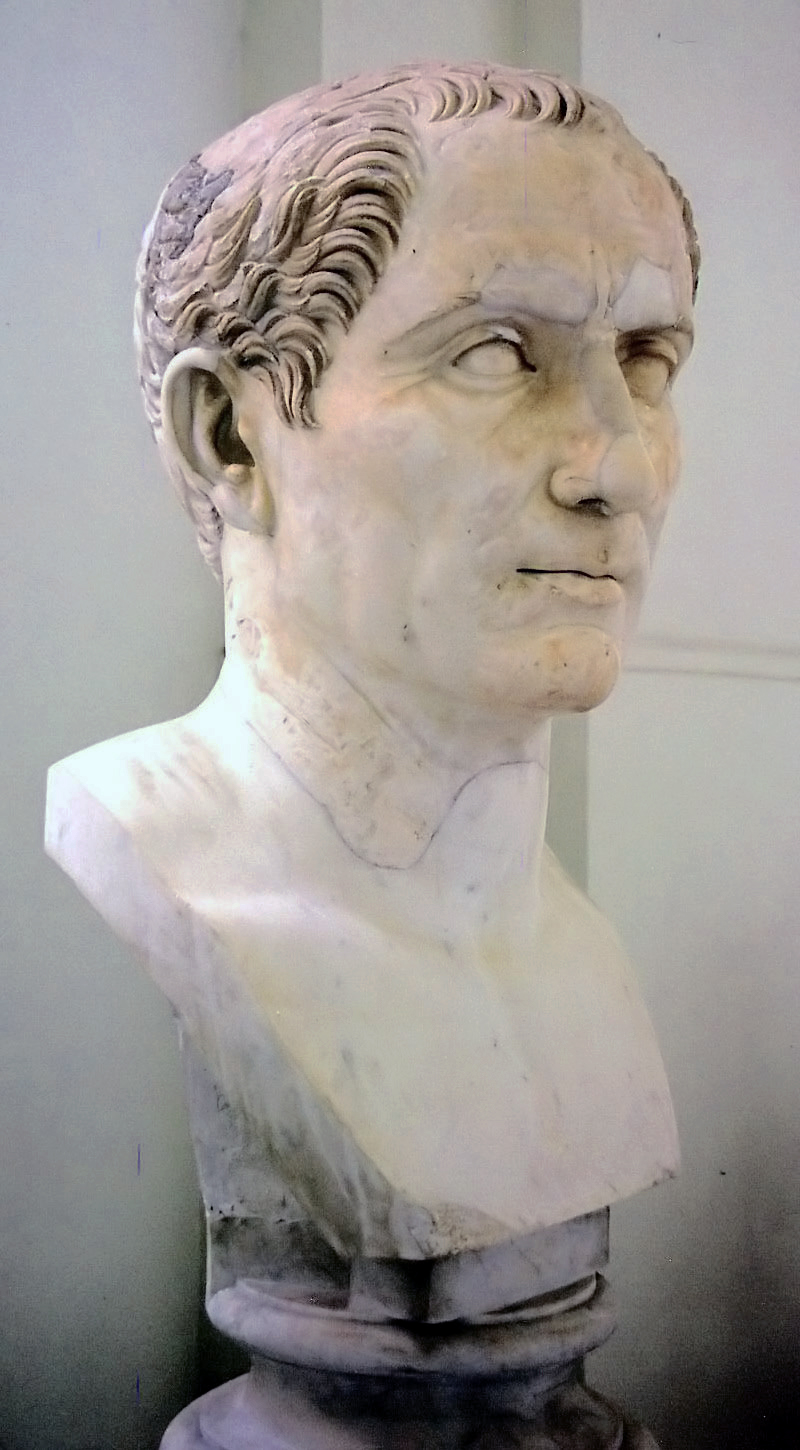
\includegraphics[width=\linewidth]{../ressources/cesare}
\end{minipage}
\begin{quote}“L’expérience, voilà le maître en toutes choses.”\end{quote}

Préceptes
\begin{itemize}
\item stabilité militaire et logistique
\end{itemize}
Axes stratégiques
\begin{enumerate}
\item infanterie lourde
\item bataillons étrangers spécialisés
\item formations en fonction des conditions géographiques
\item bivouac fortifié
\end{enumerate}
\cite{caesar_wiki, caesar_lacks}

\subsubsection{Genghis Khan}
Mongolie (\siecle{12})
\hfill \begin{minipage}{5cm}
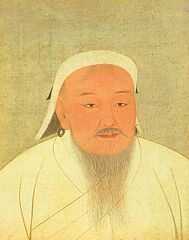
\includegraphics[width=\linewidth]{../ressources/genghis_khan}
\end{minipage}
\begin{quote}“Le plus grand bonheur du Mongol est de vaincre l’ennemi, de ravir ses trésors, de faire hurler ses serviteurs, de se sauver au galop de ses chevaux bien nourris [\ldots]”\end{quote}

Préceptes
\begin{itemize}
\item guerre psychologique
\item règne de la terreur
\item connaissance du terrain : espionnage ; éclaireurs
\end{itemize}
Axes stratégiques
\begin{enumerate}
\item peu de troupes ; avant-garde forte
\item troupes montées % logistique et vitesse
\item délégation des décisions
\item relais de communication et ravitaillement
\item attaques biologiques
\end{enumerate}
\cite{khan_wiki, military_strategy, mongol_army}

\subsubsection{Napoléon Bonaparte}
France (\siecle{18})
\hfill \begin{minipage}{5cm}
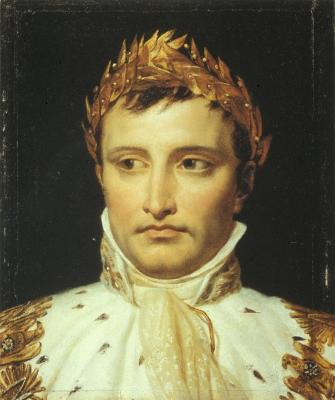
\includegraphics[width=\linewidth]{../ressources/napoleon}
\end{minipage}
\begin{quote}“Réunir ses feux contre un seul point ; une fois la brèche faite, l’équilibre est rompu, tout le reste devient inutile.”\end{quote}
Préceptes
\begin{itemize}
\item recherche systématique de la bataille
\item destruction totale des forces adverses
\item être le plus fort à l’endroit où l’on a décidé de frapper le coup décisif
\end{itemize}
Axes stratégiques
\begin{enumerate}
\item vitesse de manœuvre : {\emph Blitzkrieg}
\item fortifications
\item lignes de réapprovisionnement provisoires
\item artillerie
\end{enumerate}
\cite{napoleon, napoleon_wiki, napoleon_portrait}


\subsubsection{Conclusion}

\begin{tabular}{|p{0.45\linewidth}|p{0.45\linewidth}|}
\hline
\emph{Stratégie indirecte} & \emph{Stratégie directe}\\
\hline
renseignement & conscription\\
embuscade & recherche de la bataille décisive\\
tromperie & planification et formations\\
sabotage & fortifications\\
\hline
\end{tabular}

\begin{figure}[H]
	\begin{centering}
	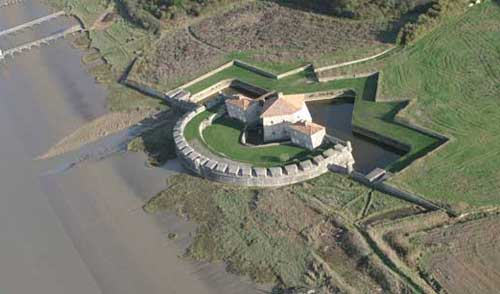
\includegraphics[width=0.8\linewidth]{../ressources/Vauban_Fort_Lupin}
	\caption{Vue aérienne du Fort Lupin construit par Vauban (Rochefort). \cite{fort_lupin}}
	\end{centering}
\end{figure}
\begin{figure}[H]
	\begin{centering}
	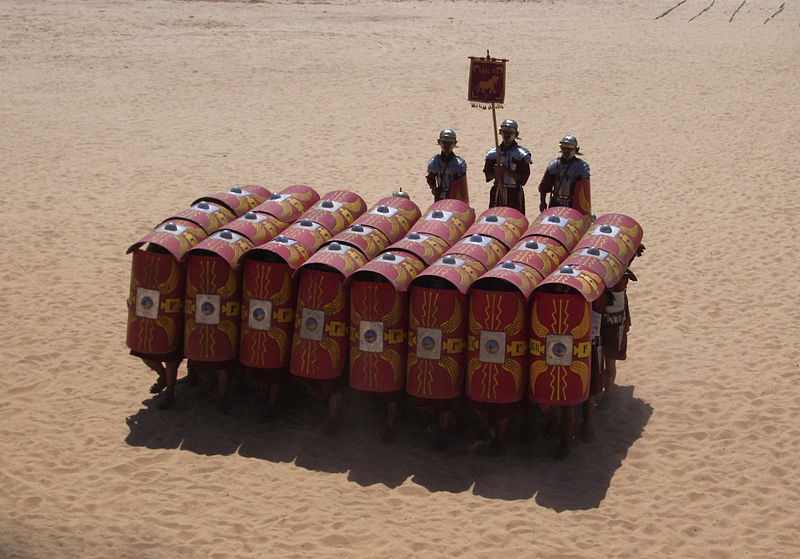
\includegraphics[width=\linewidth]{../ressources/tortue}
	\caption{La tortue : formation défensive romaine. \cite{turtle_form}}
	\end{centering}
\end{figure}
\begin{figure}[H]
	\begin{centering}
	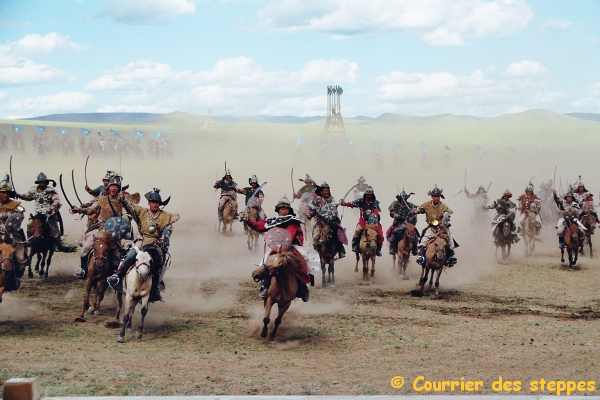
\includegraphics[width=\linewidth]{../ressources/mongol_army}
	\caption{Charge de cavalerie mongole. \cite{mongol_cavalery}}
	\end{centering}
\end{figure}
\begin{figure}[H]
	\begin{centering}
	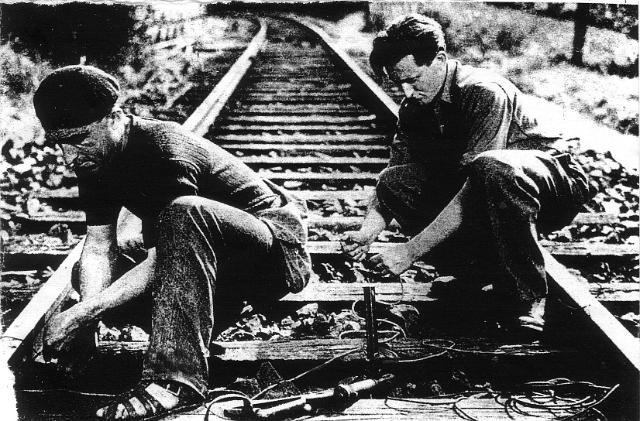
\includegraphics[width=\linewidth]{../ressources/sabotage_maquisards}
	\caption{Sabotage d'une voie de chemin de fer - guerre de 1914. \cite{sabotage}}
	\end{centering}
\end{figure}
\cite{war}


\subsection{Formations et unités}

\subsubsection{Infanterie}
\begin{figure}[H]
	\begin{centering}
	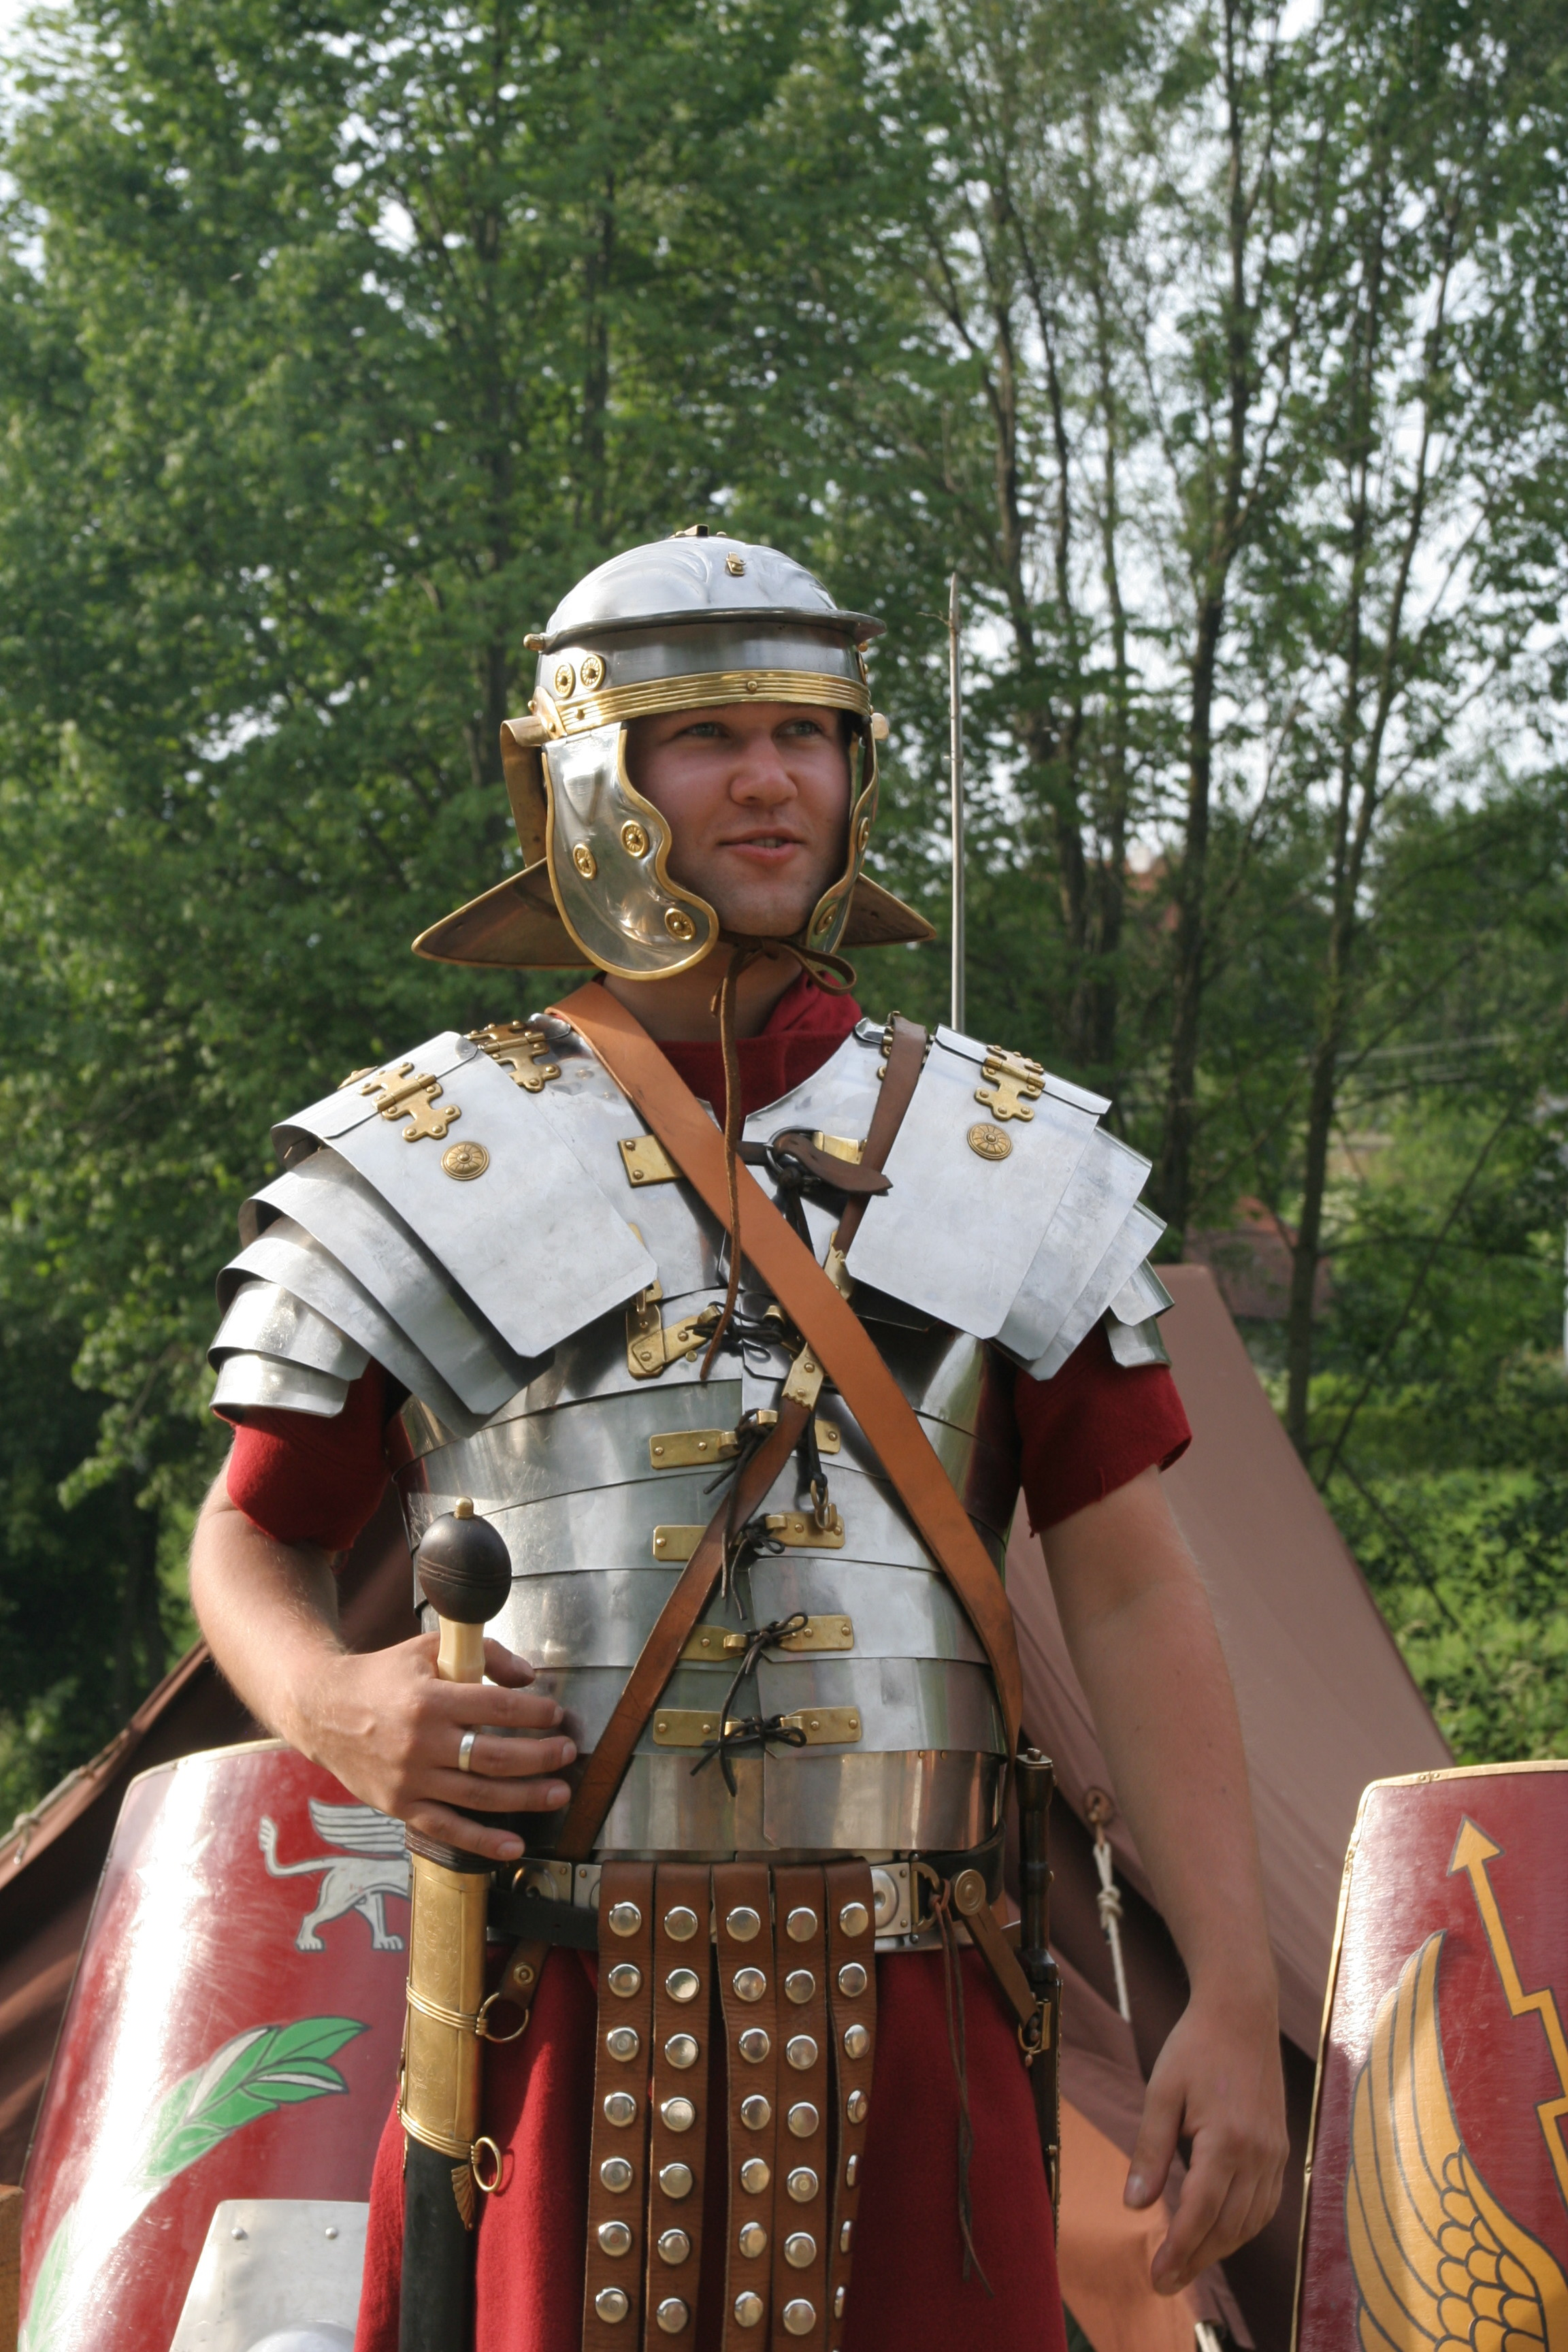
\includegraphics[width=0.42\paperwidth]{../ressources/Roman_soldier}
	\caption{Uniforme d'un légionnaire romain du \siecle{1} siècle. \cite{infantery}}
	\end{centering}
\end{figure}
\begin{figure}[H]
	\begin{centering}
	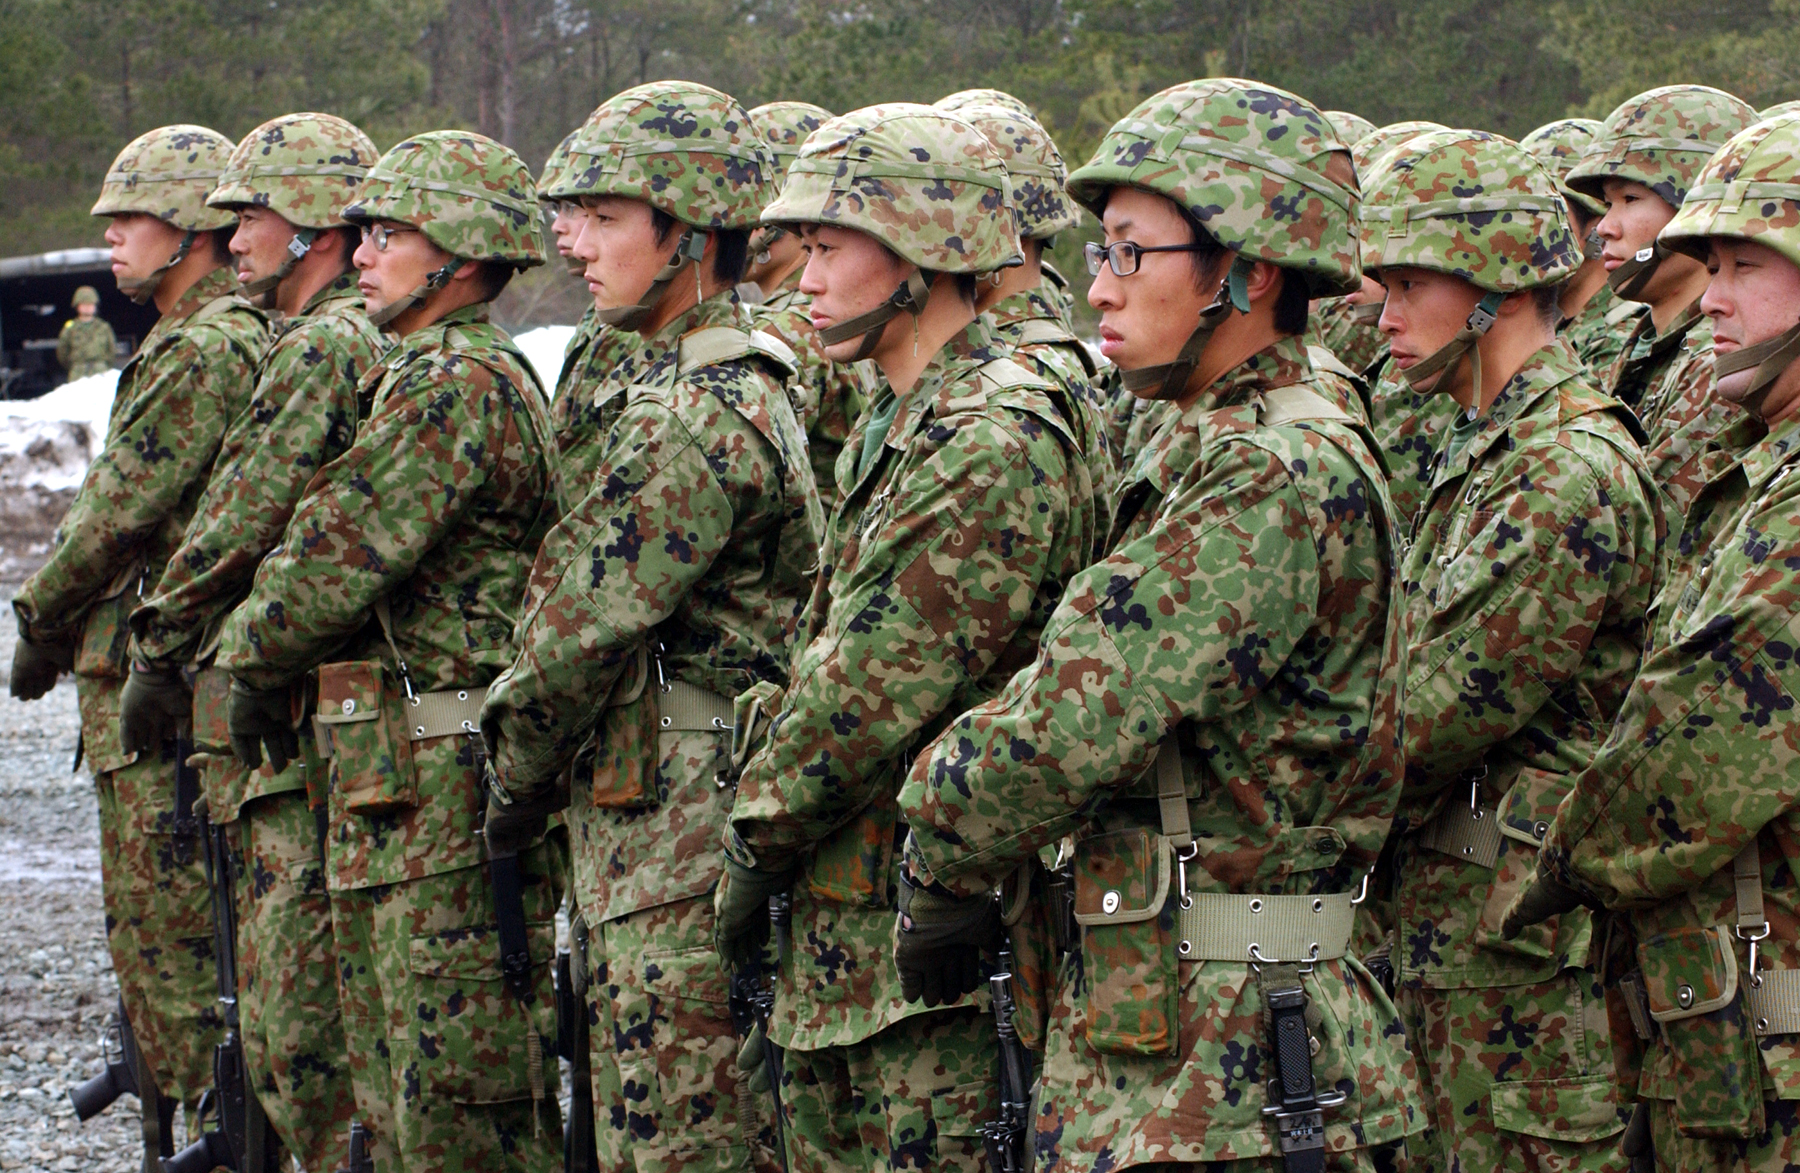
\includegraphics[width=0.55\paperwidth]{../ressources/JGDSF_Soldiers}
	\caption{Japan Ground Self-Defense Force infantry. \cite{infantery}}
	\end{centering}
\end{figure}

\subsubsection{Cavalerie légère}
\begin{figure}[H]
	\begin{centering}
	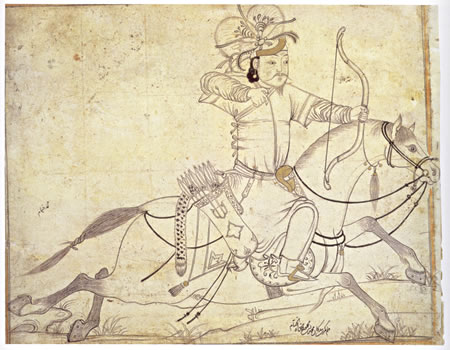
\includegraphics[width=0.5\paperwidth]{../ressources/IlkhanidHorseArcher}
	\caption{Archer à cheval Houlagides. \cite{archery}}
	\end{centering}
\end{figure}
\begin{figure}[H]
	\begin{centering}
	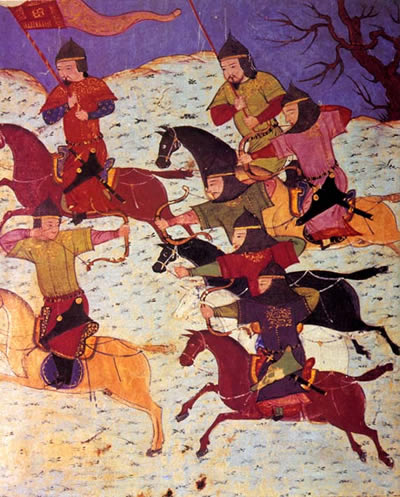
\includegraphics[width=0.47\paperwidth]{../ressources/MongolCavalrymen}
	\caption{Archers mongoles à cheval au combat (illustration d'un manuscrit du début du xive siècle) \cite{mongol_army}}
	\end{centering}
\end{figure}


\subsubsection{Cavalerie lourde}
\begin{figure}[H]
	\begin{centering}
	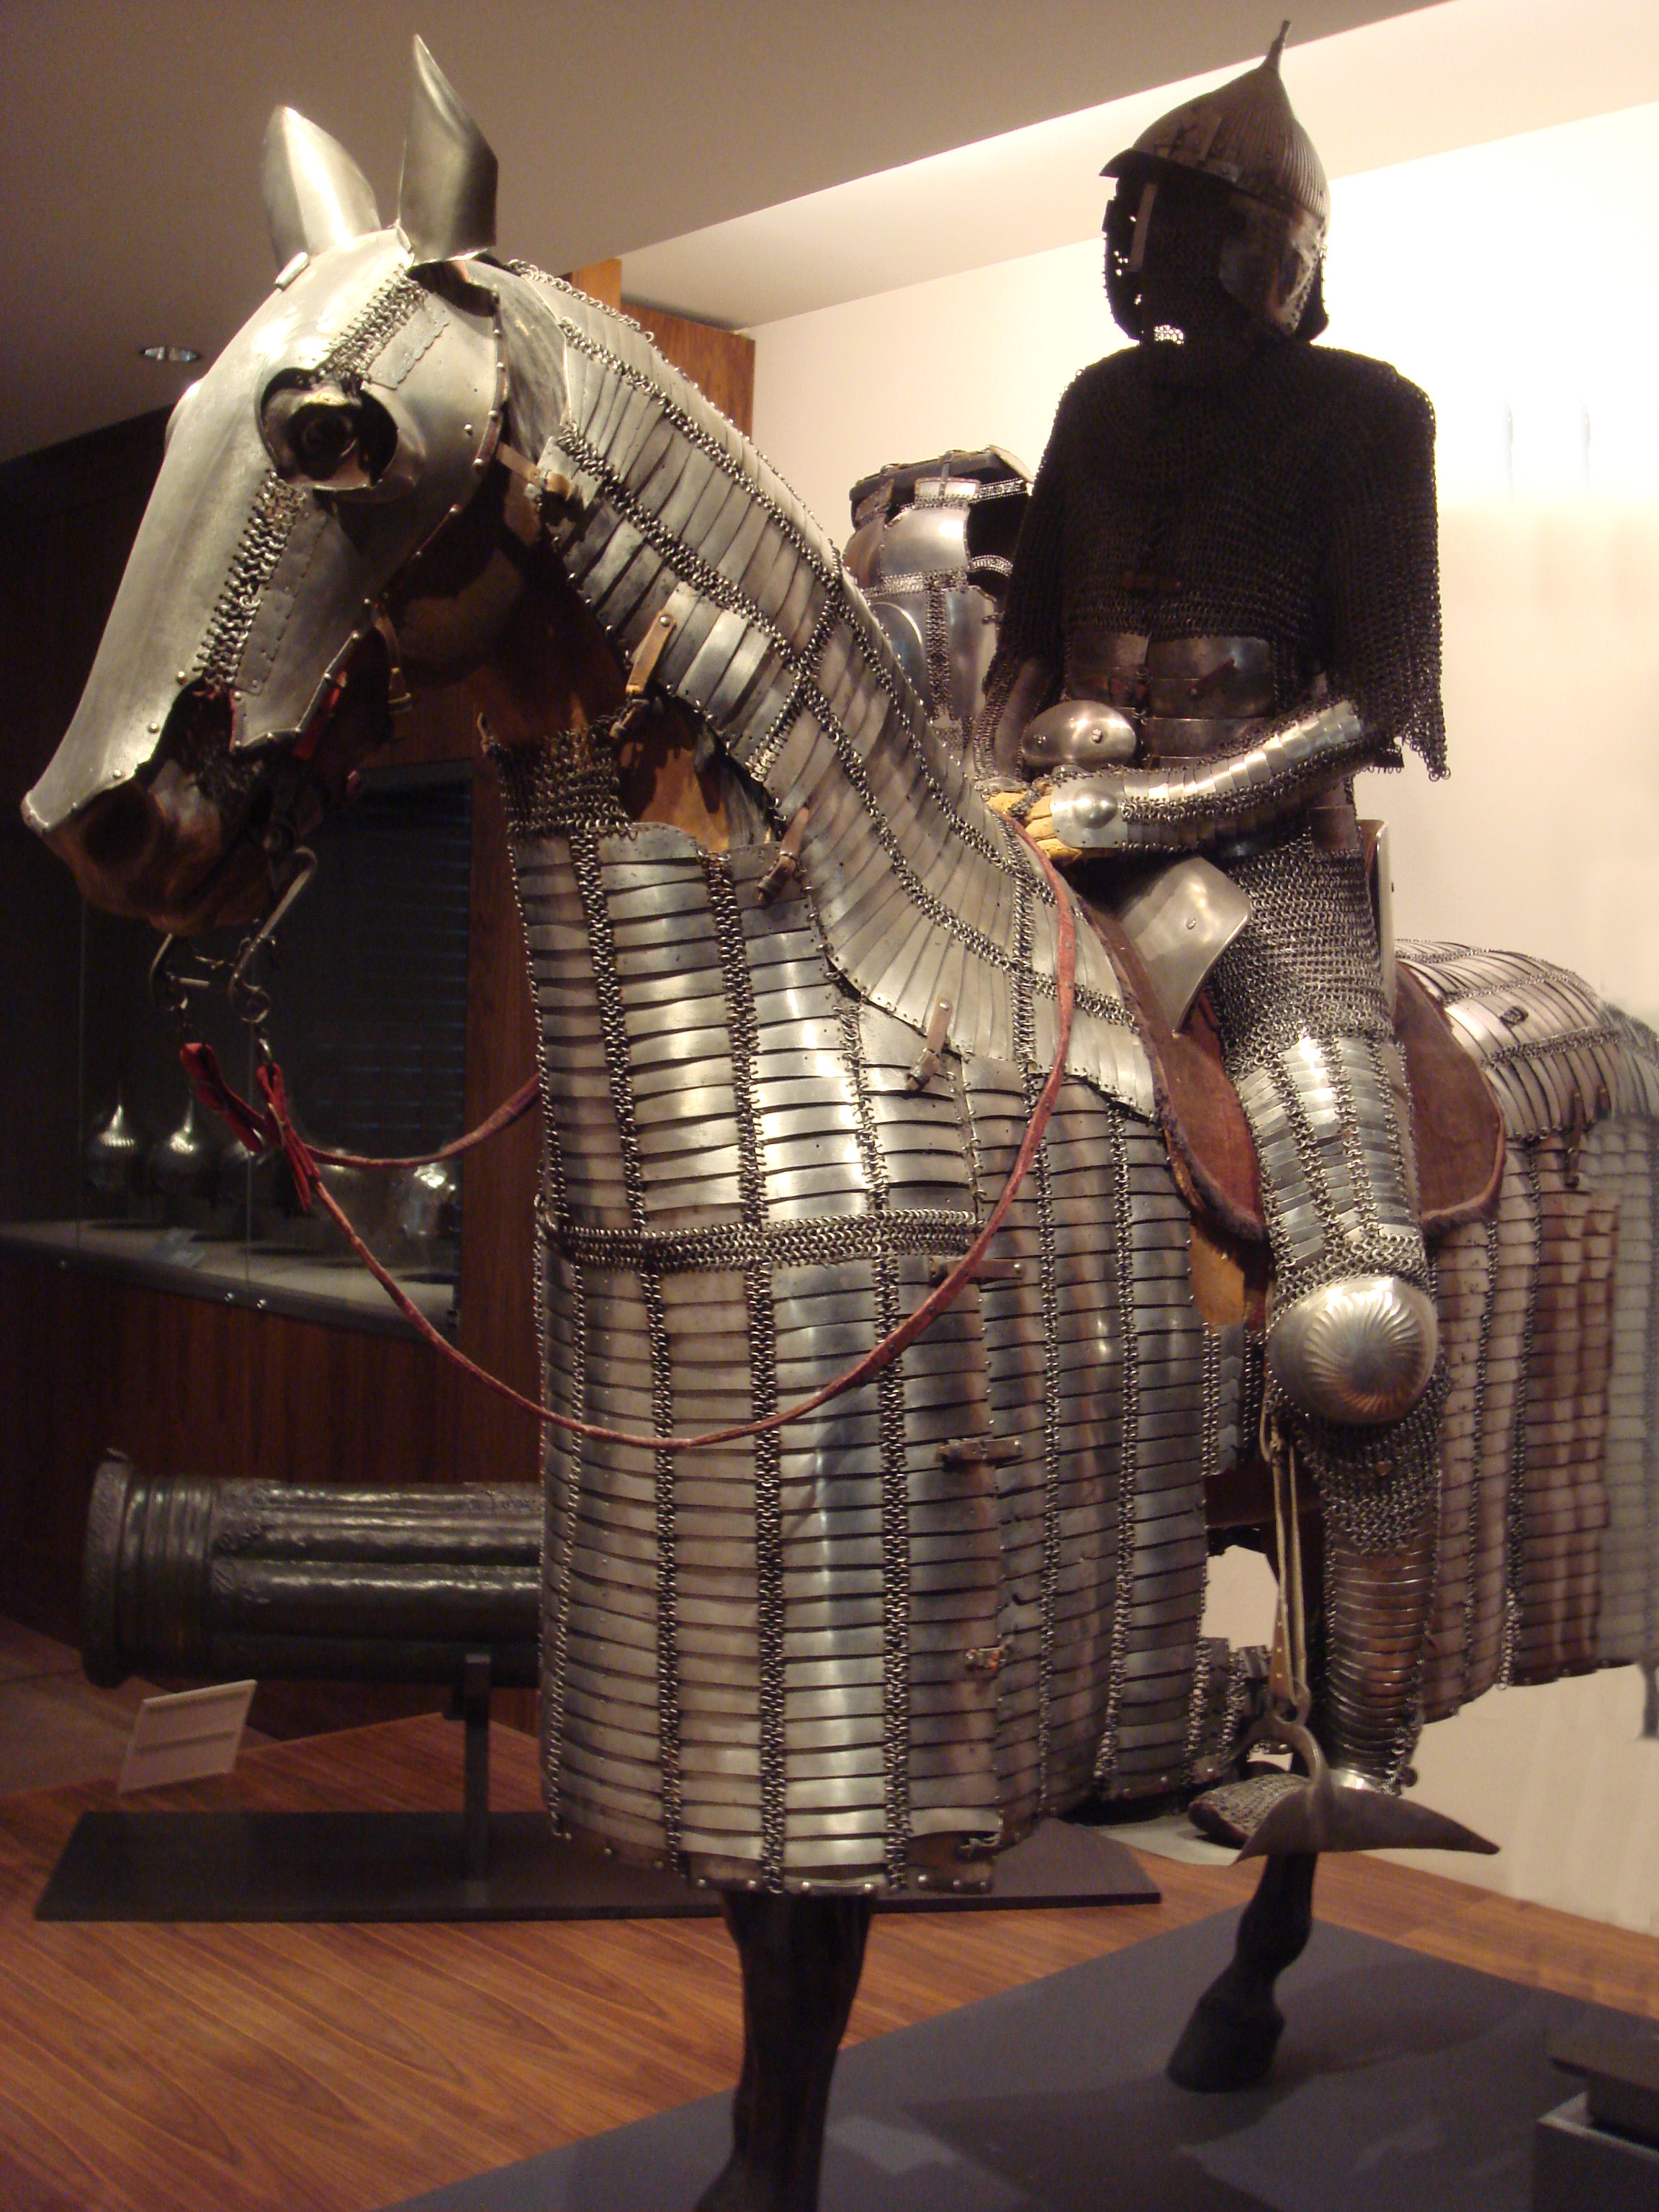
\includegraphics[width=0.44\paperwidth]{../ressources/Ottoman_Mamluk_horseman}
	\caption{Ottoman Mamluk heavy cavalry, circa 1550. \cite{heavy_cavalry}}
	\end{centering}
\end{figure}
\begin{figure}[H]
	\begin{centering}
	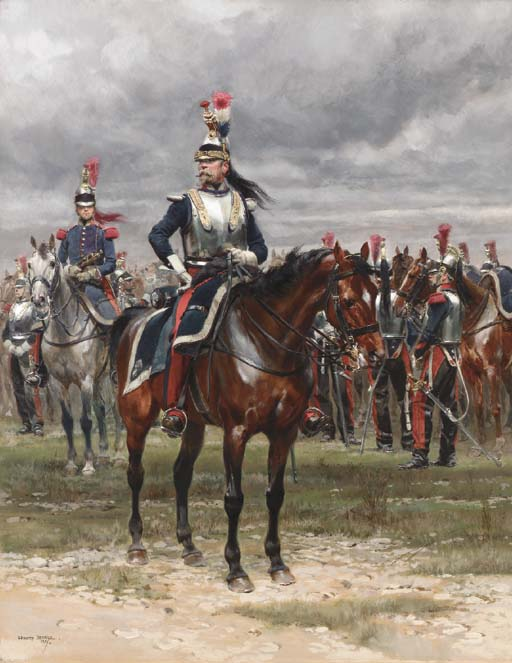
\includegraphics[width=0.5\paperwidth]{../ressources/cuirassiers}
	\caption{French cuirassiers, 19th century \cite{heavy_cavalry}}
	\end{centering}
\end{figure}

\subsubsection{Formation en triple ligne}
\begin{figure}[H]
	\begin{centering}
	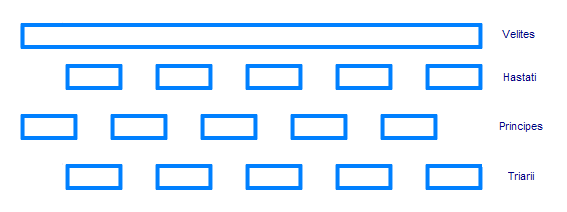
\includegraphics[width=\linewidth]{../ressources/Polybian_formation}
	\caption{Disposition classique en trois lignes \cite{roman_infantry_tactics}}
	\end{centering}
\end{figure}
\begin{figure}[H]
	\begin{centering}
	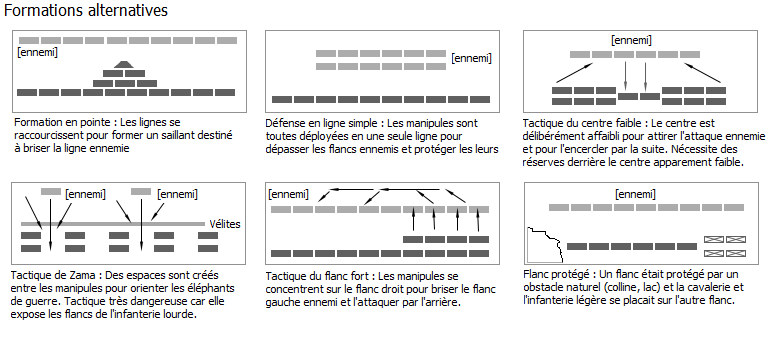
\includegraphics[width=\linewidth]{../ressources/Formations_infanterie_romaine}
	\caption{Formations alternatives \cite{roman_infantry_tactics}}
	\end{centering}
\end{figure}



\subsection{Tactiques}

\subsubsection{Charge}
\begin{figure}[H]
	\begin{centering}
	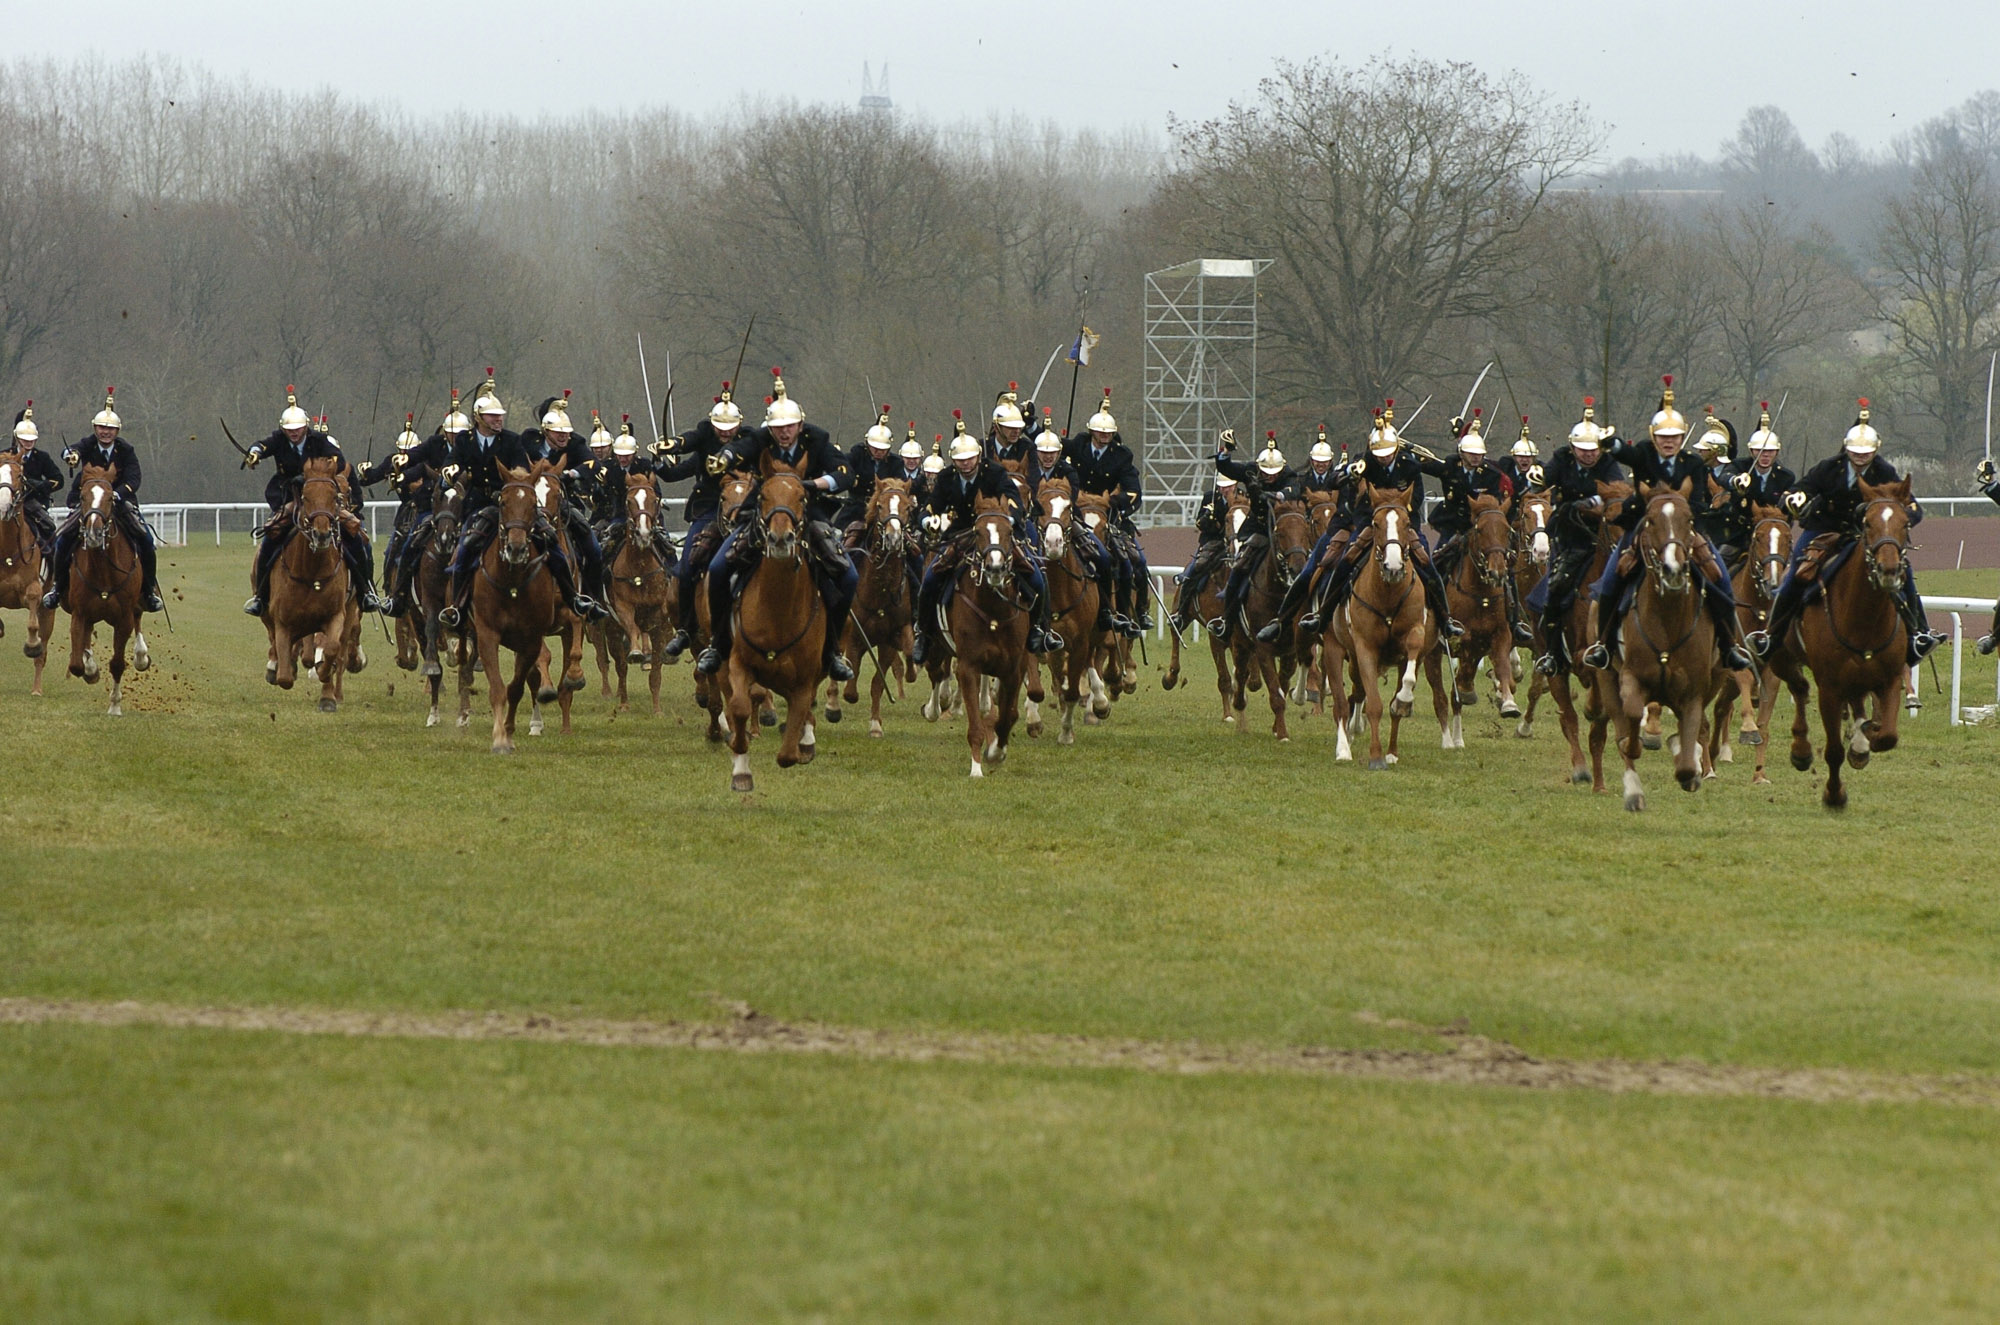
\includegraphics[width=\linewidth]{../ressources/Charge-de-cavalerie}
	\caption{Charge de cavalerie de la garde républicaine \cite{charge_cavalery}}
	\end{centering}
\end{figure}
\begin{figure}[H]
	\begin{centering}
	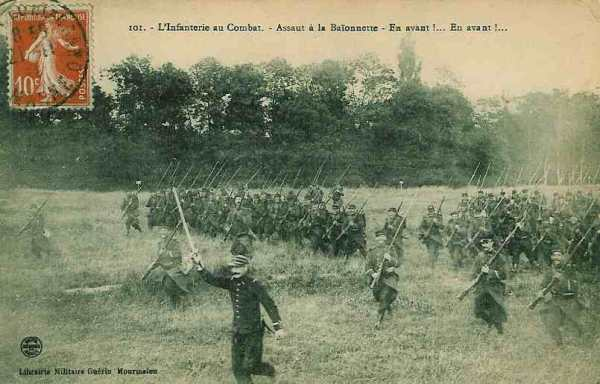
\includegraphics[width=\linewidth]{../ressources/charge_infanterie}
	\caption{Charge d’infanterie française 1914 \cite{infantery_charge}}
	\end{centering}
\end{figure}
\cite{charge_tactic}

\subsubsection{Manœuvre de flanquement}
\begin{figure}[H]
	\begin{centering}
	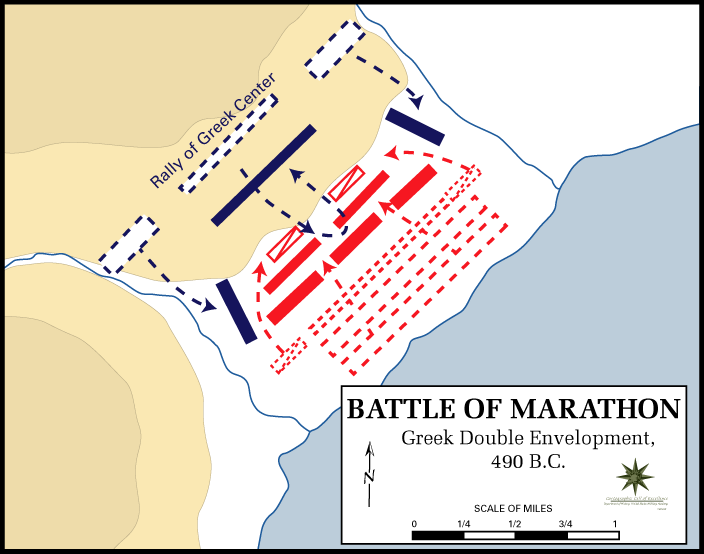
\includegraphics[width=\linewidth]{../ressources/Battle_of_Marathon}
	\caption{Bataille de Marathon (double enveloppement, manœuvre de flanquement) \cite{flanking_maneuver}}
	\end{centering}
\end{figure}
\begin{figure}[H]
	\begin{centering}
	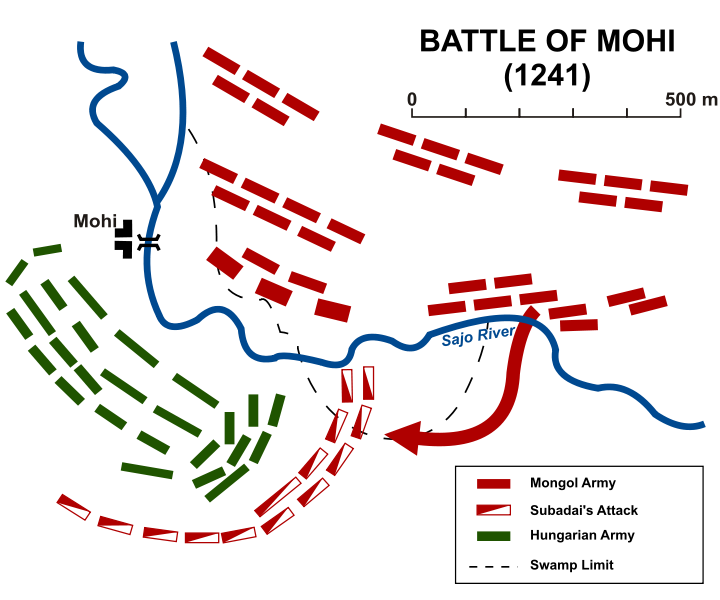
\includegraphics[width=\linewidth]{../ressources/Battle_of_Mohi}
	\caption{Plan de la bataille de Mohi (Hongrie) \cite{mohi_battle}}
	\end{centering}
\end{figure}
\cite{tactic,pincer_tactic}

\subsubsection{Le marteau et l'enclume}
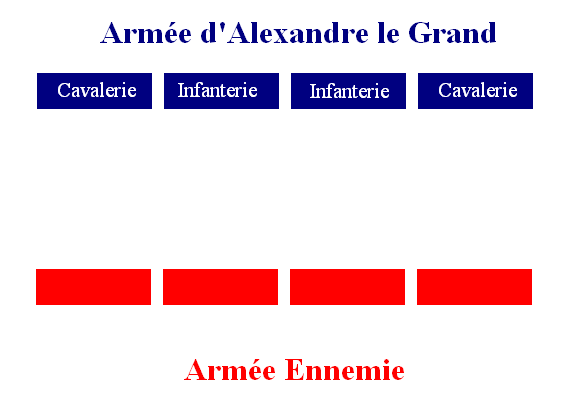
\includegraphics[width=\linewidth]{../ressources/marteau}
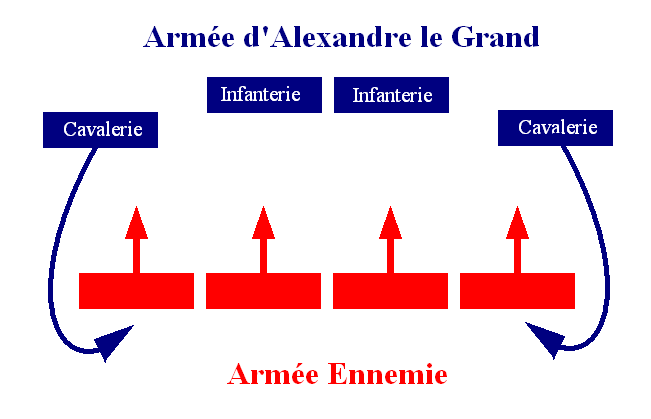
\includegraphics[width=\linewidth]{../ressources/marteau2}
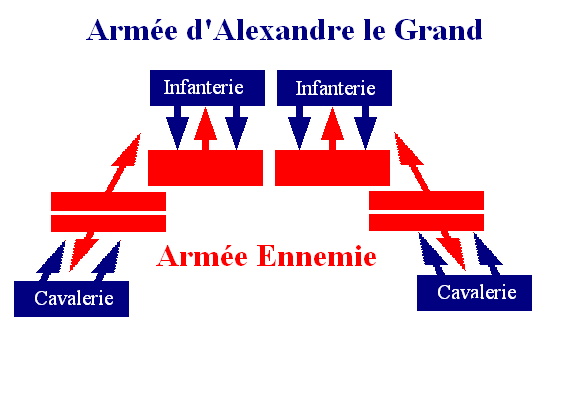
\includegraphics[width=\linewidth]{../ressources/enclume}
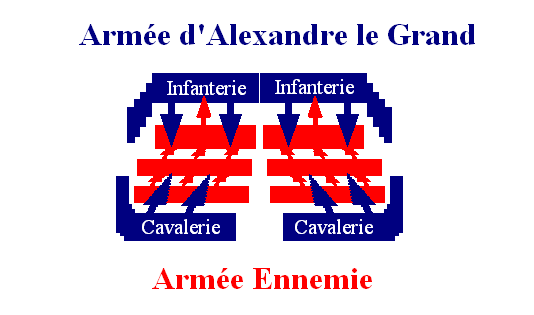
\includegraphics[width=\linewidth]{../ressources/enclume2}
\cite{Alexanders_tactics}

\subsubsection{Contre-attaque}
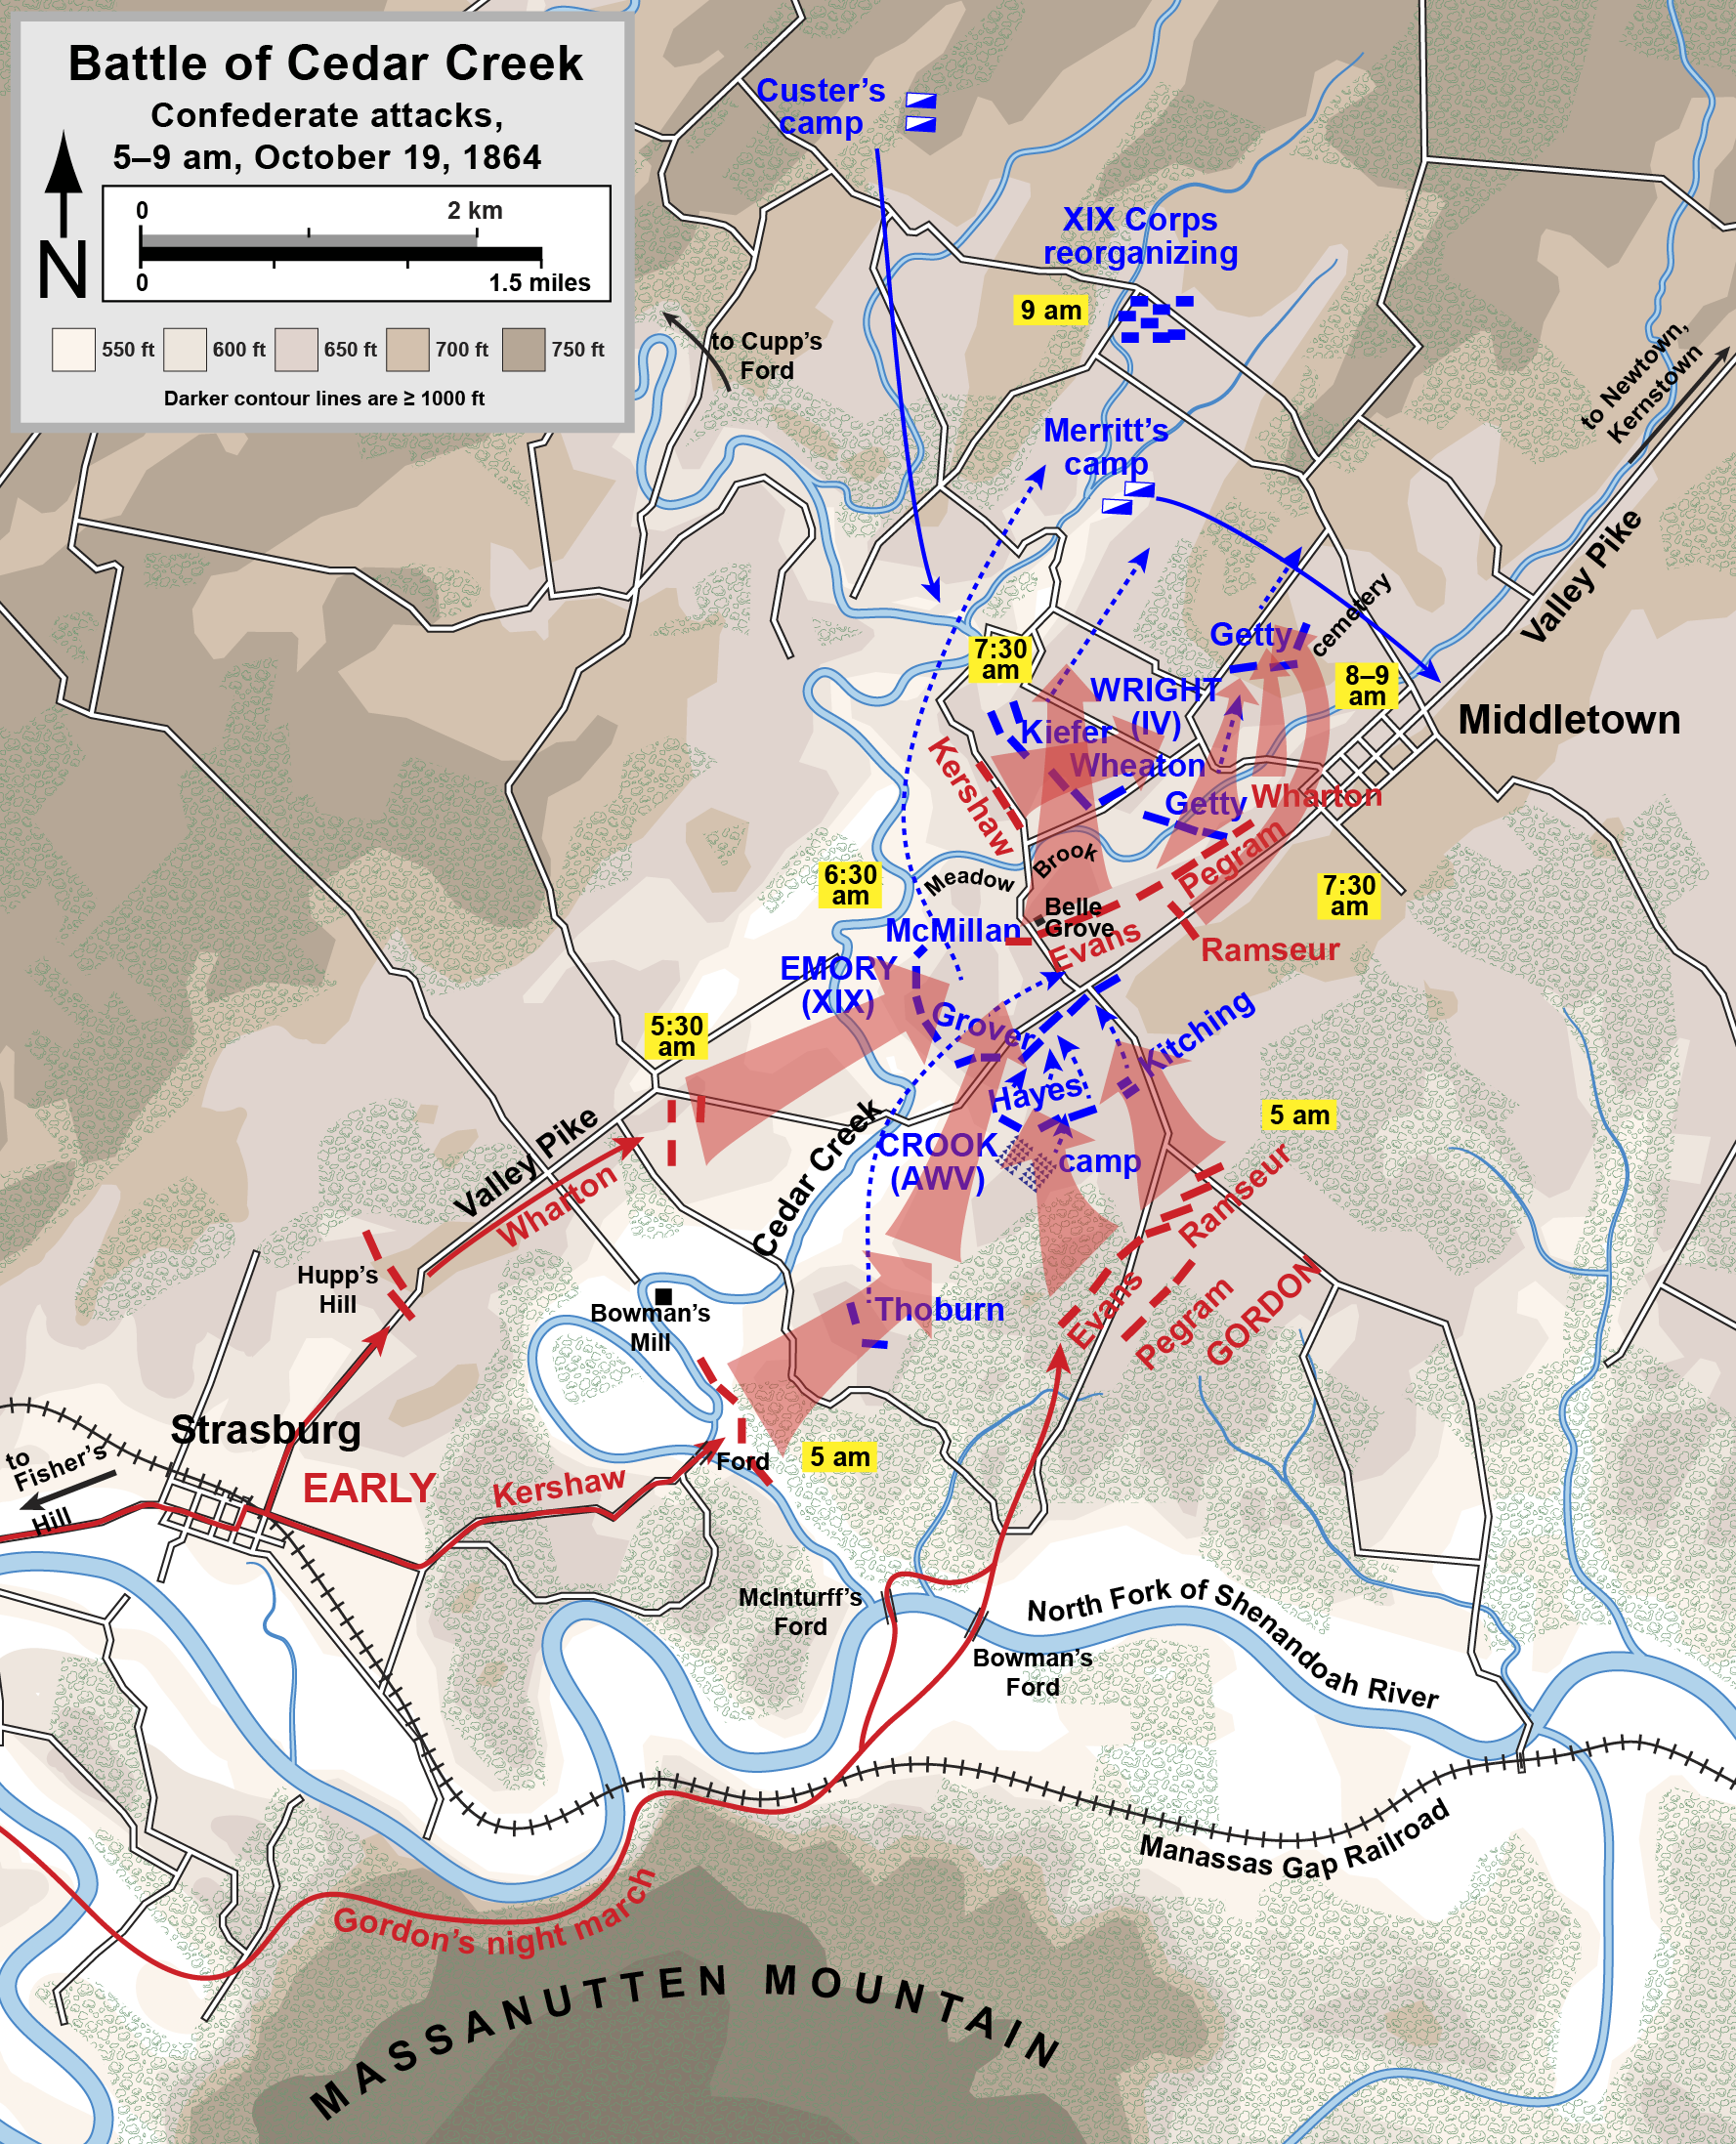
\includegraphics[width=\linewidth]{../ressources/Cedar_Creek_Confederate_attacks}
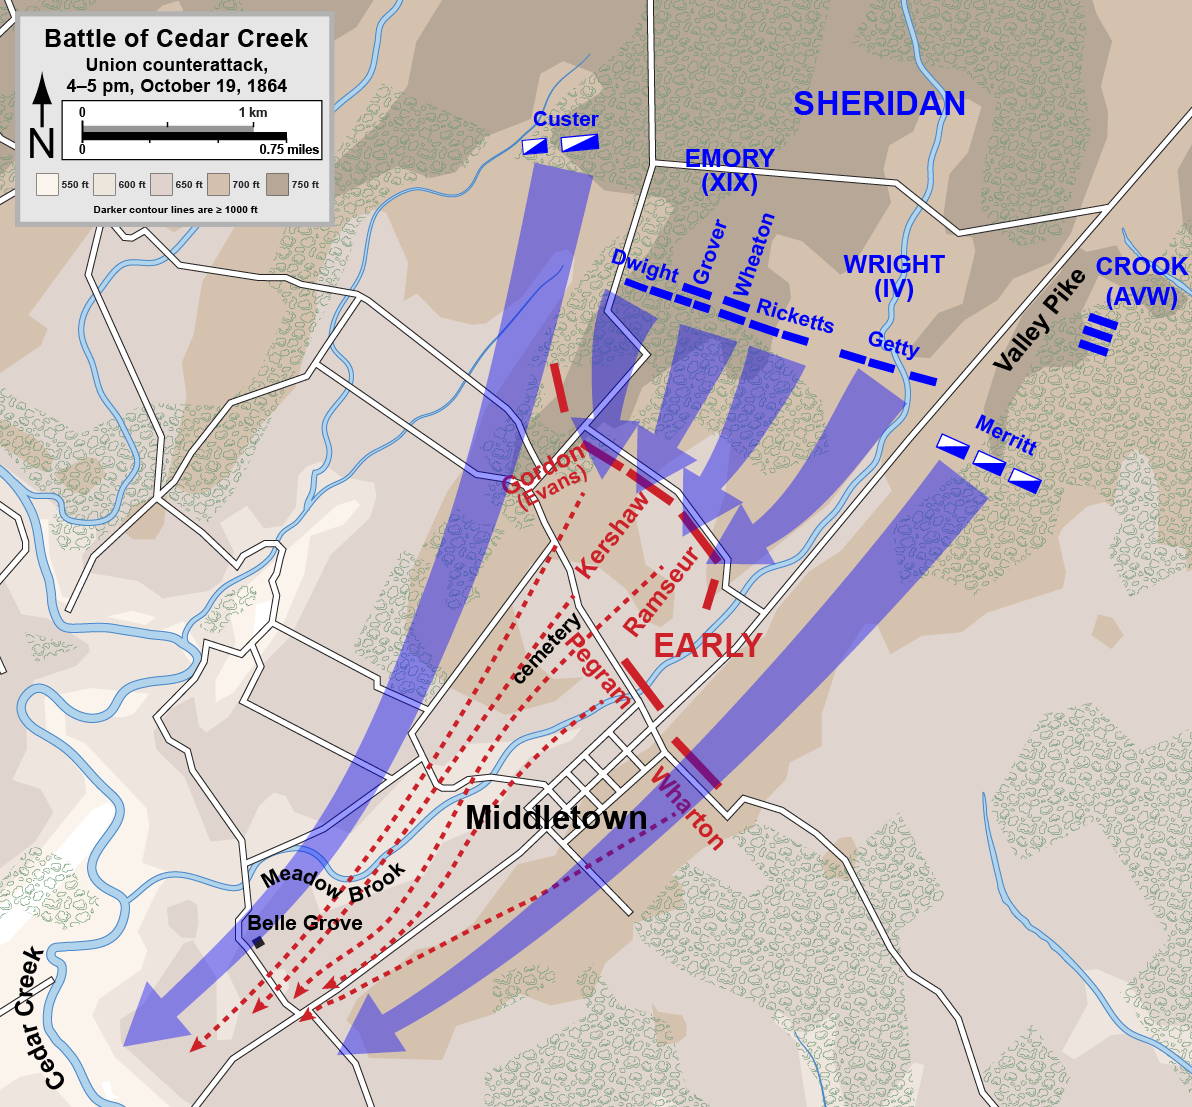
\includegraphics[width=\linewidth]{../ressources/Cedar_Creek_Union_counterattack}
\cite{counterattack_wiki, couterattack_cedar_creek}

\subsubsection{Retraite feinte}
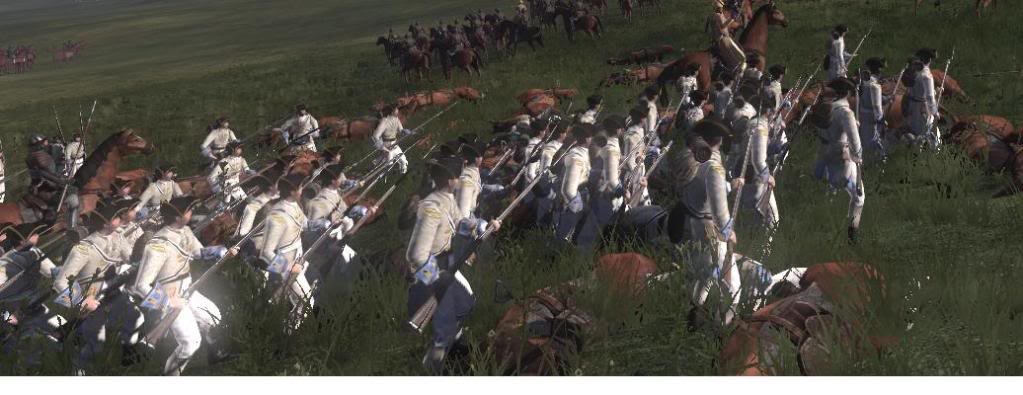
\includegraphics[width=\linewidth]{../ressources/infantrysquare3}
\cite{mongol_army,feigned_retreat}


\subsubsection{Embuscade}
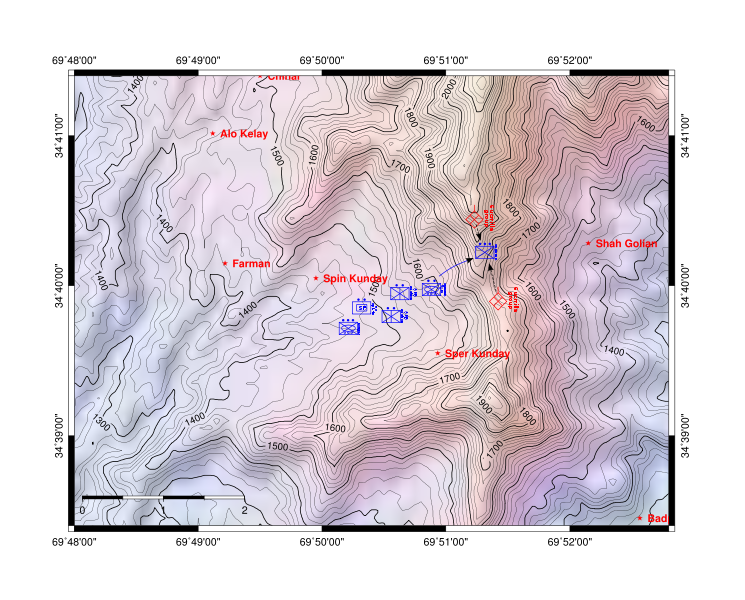
\includegraphics[width=\linewidth]{../ressources/Uzbin_valley_ambush-map}
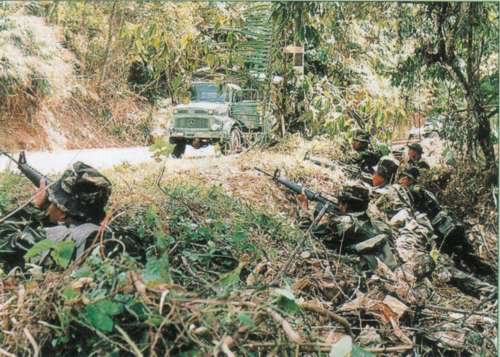
\includegraphics[width=\linewidth]{../ressources/ambush}
\cite{ambush_wiki, uzbin_ambush, ambush_picture}

\subsubsection{Hit and run}




\section{Applications aux systèmes multi-agents}

\subsection{Enhanced Isaac Neural Simulation Toolkit (EINSTein)}
an Artificial-Life Laboratory for Exploring Self-Organized Emergence in Land Combat
Andy Ilachinski

\includegraphics[]{../ressources/ilachinski}
1999
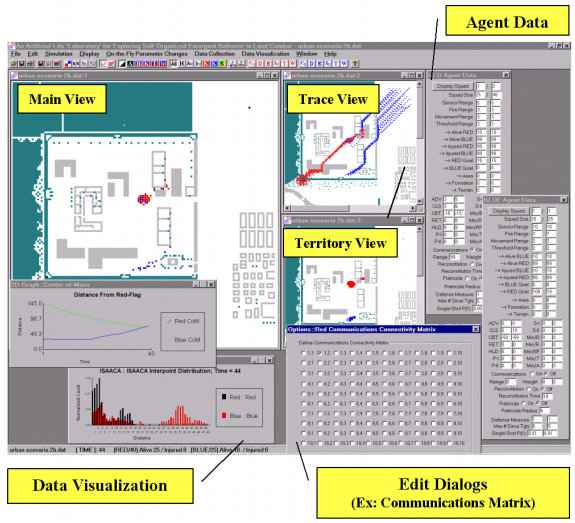
\includegraphics[width=\linewidth]{../ressources/Einstein}
\cite{simu_guerre,ilachinski1994,ilachinski1999}

motivation des agents
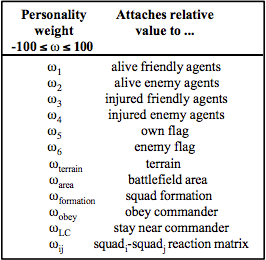
\includegraphics[]{../ressources/einstein_personality_weight}
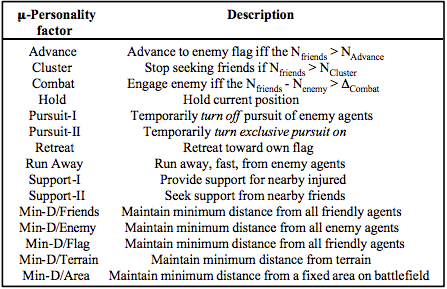
\includegraphics[]{../ressources/einstein_personality_factor}

émergence d'un comportement global
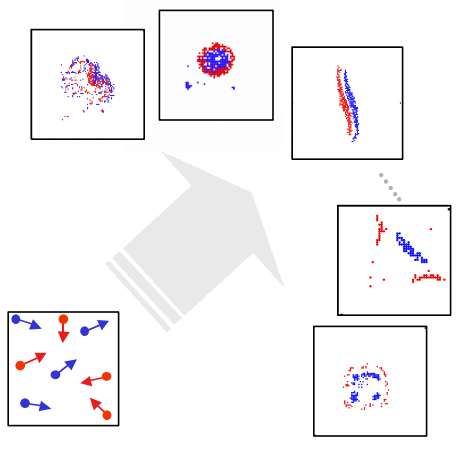
\includegraphics[]{../ressources/einstein_global_behavior}
formation en pointe
encerclement
assault frontal
prise en tenaille
guérilla

\subsection{Iruba}
An Agent-Based Model of the Guerrilla War Process
Jim Doran
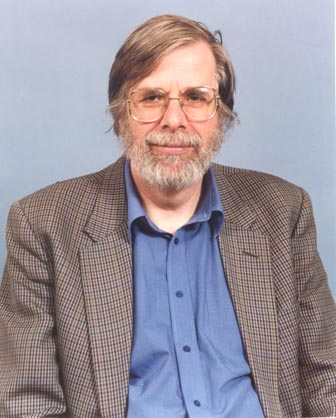
\includegraphics[]{../ressources/doran}
2005
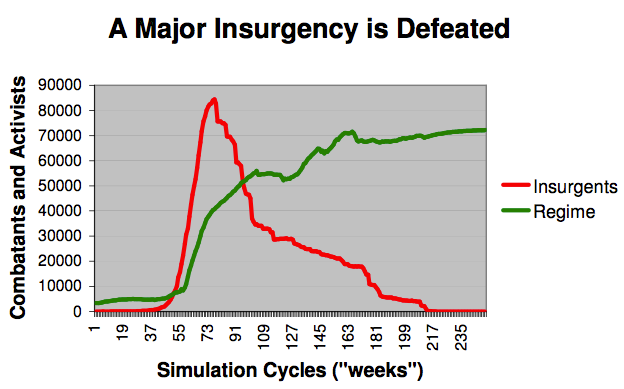
\includegraphics[]{../ressources/insurgency}
\begin{algorithmic}[1]
		\WHILE{non termination}
			\STATE Attacks and their impact
			\STATE HQ decisions
			\STATE Recruitment
			\STATE Force movement
		\ENDWHILE
		\end{algorithmic}
\cite{doran2005iruba}

Stratégies influant sur la réussite
initial guerrilla band size
regime force concentration
insurgent mobility
insurgent hyper-mobility
all-out regime counter attack

Stratégies influant sur la réussite
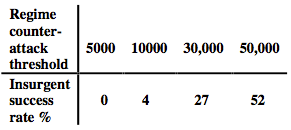
\includegraphics[scale=0.5]{../ressources/iruba_counter_attack}
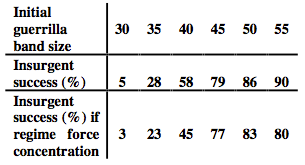
\includegraphics[scale=0.5]{../ressources/iruba_force_concentration}
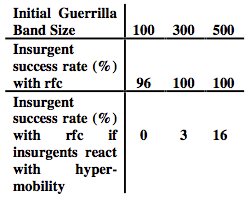
\includegraphics[scale=0.5]{../ressources/iruba_hyper_mobility}
\includegraphics[scale=0.5]{../ressources/iruba_mobility}

\subsection{RPDAgent}
Enhanced Military Decision Modeling Using a MultiAgent System Approach
John A. Sokolowski
\includegraphics[scale=0.5]{../ressources/john_sokolowski}
2003
\includegraphics[height=0.7\paperheight]{../ressources/RPDagent_uml}
\cite{sokolowski2003}


\section{Conclusion}



\bibliographystyle{plain}
\bibliography{../Bib.bib}

\end{document}


